\selectlanguage{italian}

I sistemi macroscopici realizzano l'equilibrio termodinamico bilanciando la tendenza dell'energia interna a diminuire e quella dell'entropia ad aumentare: ad alte temperature prevale il contributo entropico, a basse temperature prevale quello energetico (nei solidi gli atomi hanno posizioni fisse, dunque l'entropia è più basse rispetto ai fluidi). Sperimentalmente, infatti, si trova che quasi tutti i materiali solidificano a temperature abbastanza basse: l'unica eccezione è l'elio, che rimane fluido fino a $ T \approx 0 \,\text{K} $, a meno che non si applichi una sufficiente pressione. \\
Così come la tendenza degli atomi a formare molecole (minimizzando $ V_\text{ad} $) viene misurata dalla binding energy molecolare, la tendenza di atomi/molecole a formare solidi viene misurata da una quantità analoga, l'\textit{energia di coesione}.

\section{Struttura microscopica}

Nello studio di solidi semplici, come ad esempio quelli formati da gas nobili, l'interazione tra atomi è semplificabile a coppie, quindi modellizzabile con il potenziale di Lennard-Jones:
\begin{equation}
	V_\text{ad}(\ve{R}_1 , \dots , \ve{R}_{N_n}) = \sum_{\alpha < \alpha'}^{N_n} V_2(\abs{\ve{R}_\alpha - \ve{R}_{\alpha'}})
	\qquad \qquad
	V_2(r) = 4\varepsilon \left[ \left( \frac{\sigma}{r} \right)^{12} - \left( \frac{\sigma}{r} \right)^6 \right]
\end{equation}
Per un coppia di atomi, la distanza d'equilibrio è $ R_\text{m} = \sqrt[6]{2} \sigma $ con potenziale minimo $ V_2(R_\text{m}) = -\varepsilon $. Inoltre, si vede che il potenziale decade come $ \sim r^{-6} $, quindi, contando che tipicamente il numero di atomi a distanza $ r $ da un dato atomo scala come $ \sim r^2 $, l'energia d'interazione totale a lunga distanza scala come $ r^{-4} $: si vede che ogni atomo interagisce significativamente soltanto con gli atomi ad esso vicini. \\
Si consideri un reticolo 1D di atomi: aggiungendo un terzo atomo ad una coppia di atomi, esso si posizionerà ad una distanza $ \approx R_\text{m} $ da essi (ignorando l'interazione tra secondi-vicini) ed abbasserà la buca di potenziale adiabatico a $ \approx -2\varepsilon $. Ciò è generalizzabile ad $ N_n $ atomi: essi si troveranno a distanza $ \approx R_\text{m} $ l'uno dall'altro e l'energia di coesione totale sarà $ \approx (N_n - 1) \varepsilon $ (circa $ \varepsilon $ per atomo, per $ N_n $ grande). Se si considera l'interazione con secondi- e terzi-vicini, si trova che la distanza d'equilibrio è leggermente minore rispetto a $ R_\text{m} $ e che l'energia di coesione è leggermente maggiore di $ (N_n - 1) \varepsilon $ (si veda Fig. \ref{lat-2}a). \\
Se invece si considera un reticolo 2D, il terzo atomo si posizionerà al vertice di un triangolo equilatero formato con i primi due. Aggiungendo altri atomi, si viene a formare un \textit{reticolo triangolare} (o esagonale, si veda Fig. \ref{lat-2}), in cui ciascun atomo a 6 primi-vicini, dunque l'energia di coesione sarà approssimativamente $ 3\varepsilon $ per atomo (6 legami condivisi da 2 atomi ciascuno). Si vede dunque che il modello d'interazione a coppie porta al principio di \textit{massima coordinazione}: gli atomi si dispongono in modo da massimizzare il numero di primi-vicini, così da massimizzare l'energia di coesione (minimizzando l'energia potenziale adiabatica). \\
Applicando il principio di massima coordinazione ad un reticolo 3D, si vede che 4 atomi massimizzano la loro coordinazione ponendosi ai vertici di un tetraedro regolare: gli atomi successivi si dispongono a formare o il \textit{face-centered cubic lattice} (reticolo fcc, Fig. \ref{lat-3}b) o l'\textit{hexagonal close-packed lattice} (reticolo hcp, Fig. \ref{lat-3}c). In entrambi questi reticoli ogni atomo ha 12 primi-vicini, dunque l'energia reticolare è $ 6\varepsilon $ per atomo; si vede, però, che entrambi sono formati da reticoli triangolari 2D sovrapposti: mentre nell'fcc si ripetono 3 orientazioni diverse, nell'hcp ce ne sono solo 2, dunque, quando si va a considerare l'interazione con secondi- e terzi-vicini, il reticolo fcc è leggermente favorito energeticamente rispetto all'hcp. \\
Confrontando i vari reticoli, si trovano delle distanze d'equilibrio leggermente diverse: in 1D $ R_\text{m} = \sqrt[6]{2} \sigma \simeq 1.22 \sigma $, in 2D $ R_\text{m} \simeq 1.11 \sigma $ ed in 3D $ R_\text{m} \simeq 1.09 \sigma $. Nella tavola periodica c'è una prevalenza a formare cristalli fcc ed hcp: ci sono alcuni bcc (body-centered cubic, simile all'fcc ma con un atomo al centro del cubo, al posto di quelli sulle facce) ed i casi del diamante (struttura a sé) e del polonio, che invece forma l'sc (simple cube). \\
È possibile formare strutture cristalline\footnote{Si noti che i vetri, al contrario dei cristalli, hanno una risposta plastica alle deformazioni: essi non sono solidi, ma liquidi con coefficiente di viscosità estremamente elevato, caratterizzati da livelli energetici estremamente vicini. Infatti, osservando i vedtri di edifici antichi, essi risulteranno ondulati, in quanto deformati nel tempo dalla gravità.} diverse da quelle descritte considerando un potenziale non necessariamente a 2 corpi (valido principalmente per gas nobili, che hanno interazioni deboli): potenziali a più corpi introducono effetti elettronici (quantistici) che danno direzionalità ai legami, fino ad arrivare ai solidi con legami metallici covalenti in cui le interazioni si estendono alla totalità del solido, impedendo di fattorizzare la funzione d'onda.

\begin{figure}[!h]
	\centering
	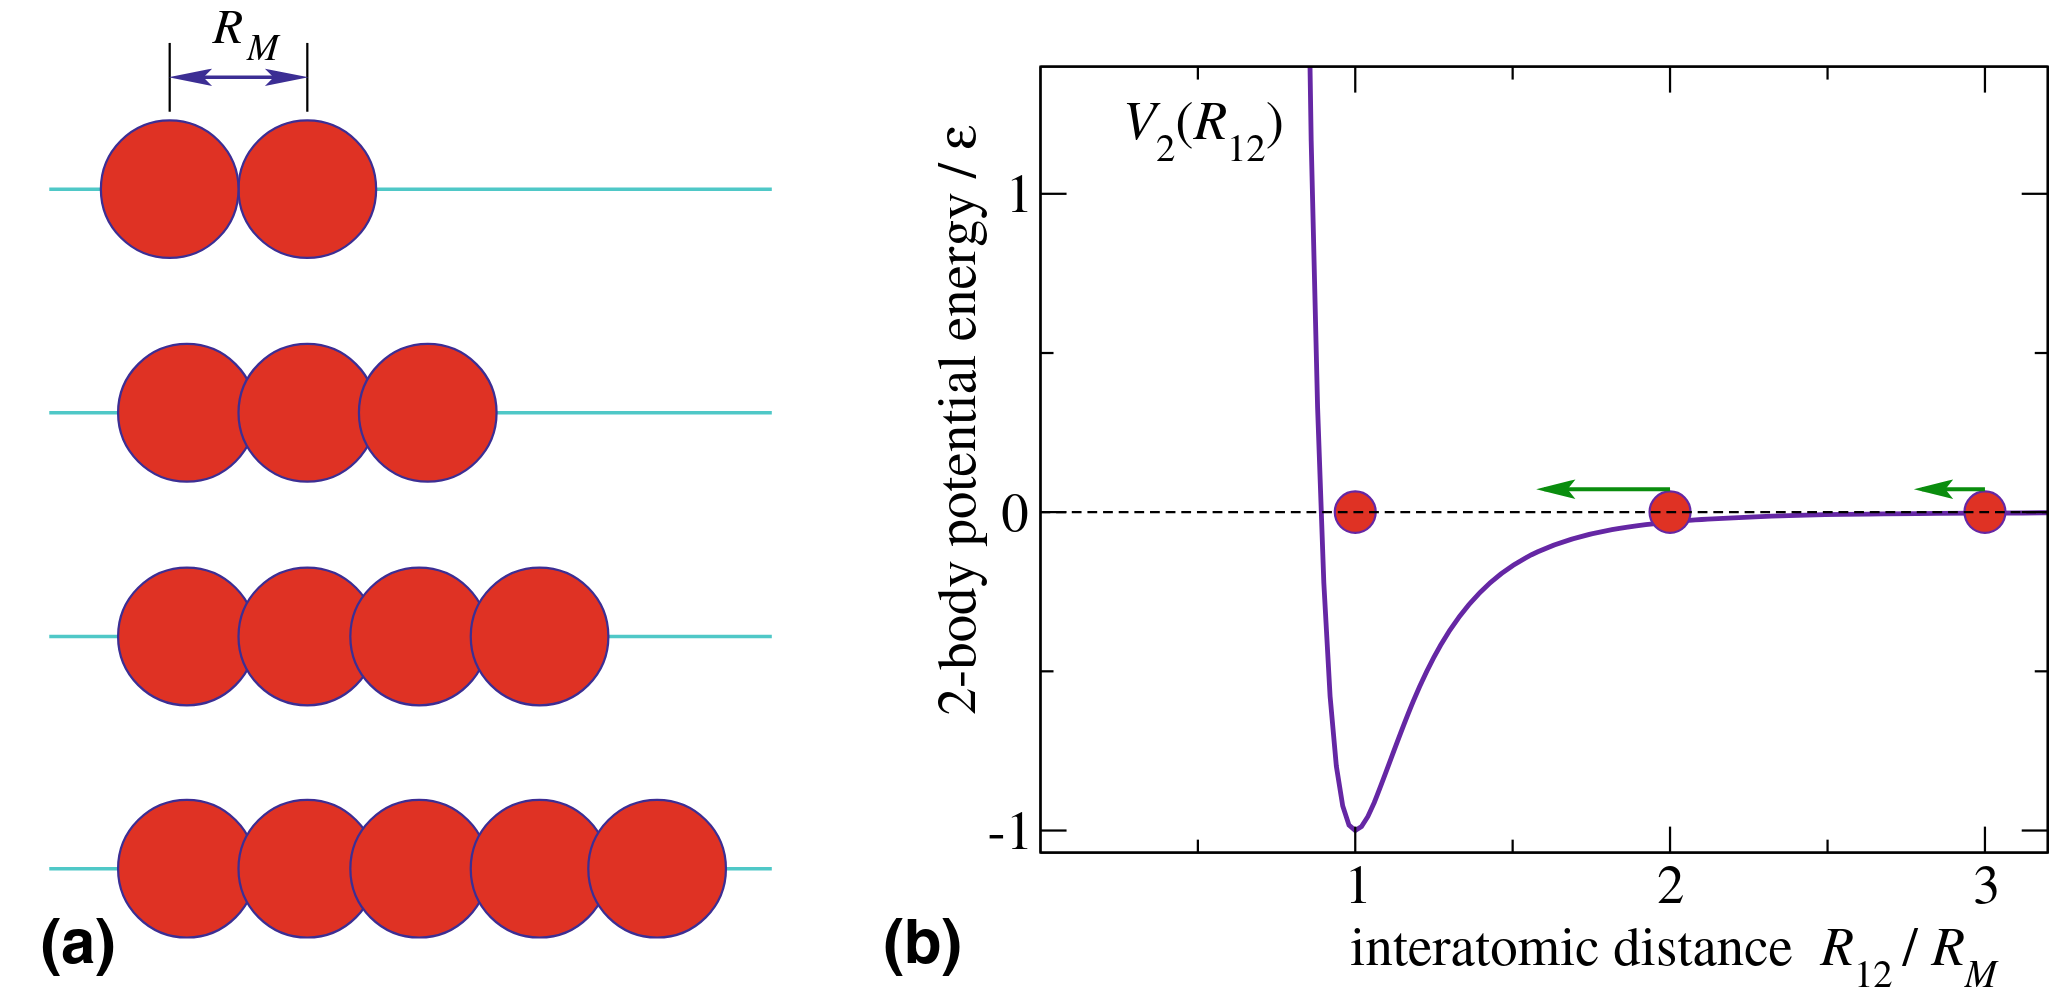
\includegraphics[width = 0.45 \textwidth]{lattice-1d.png}
	\qquad
	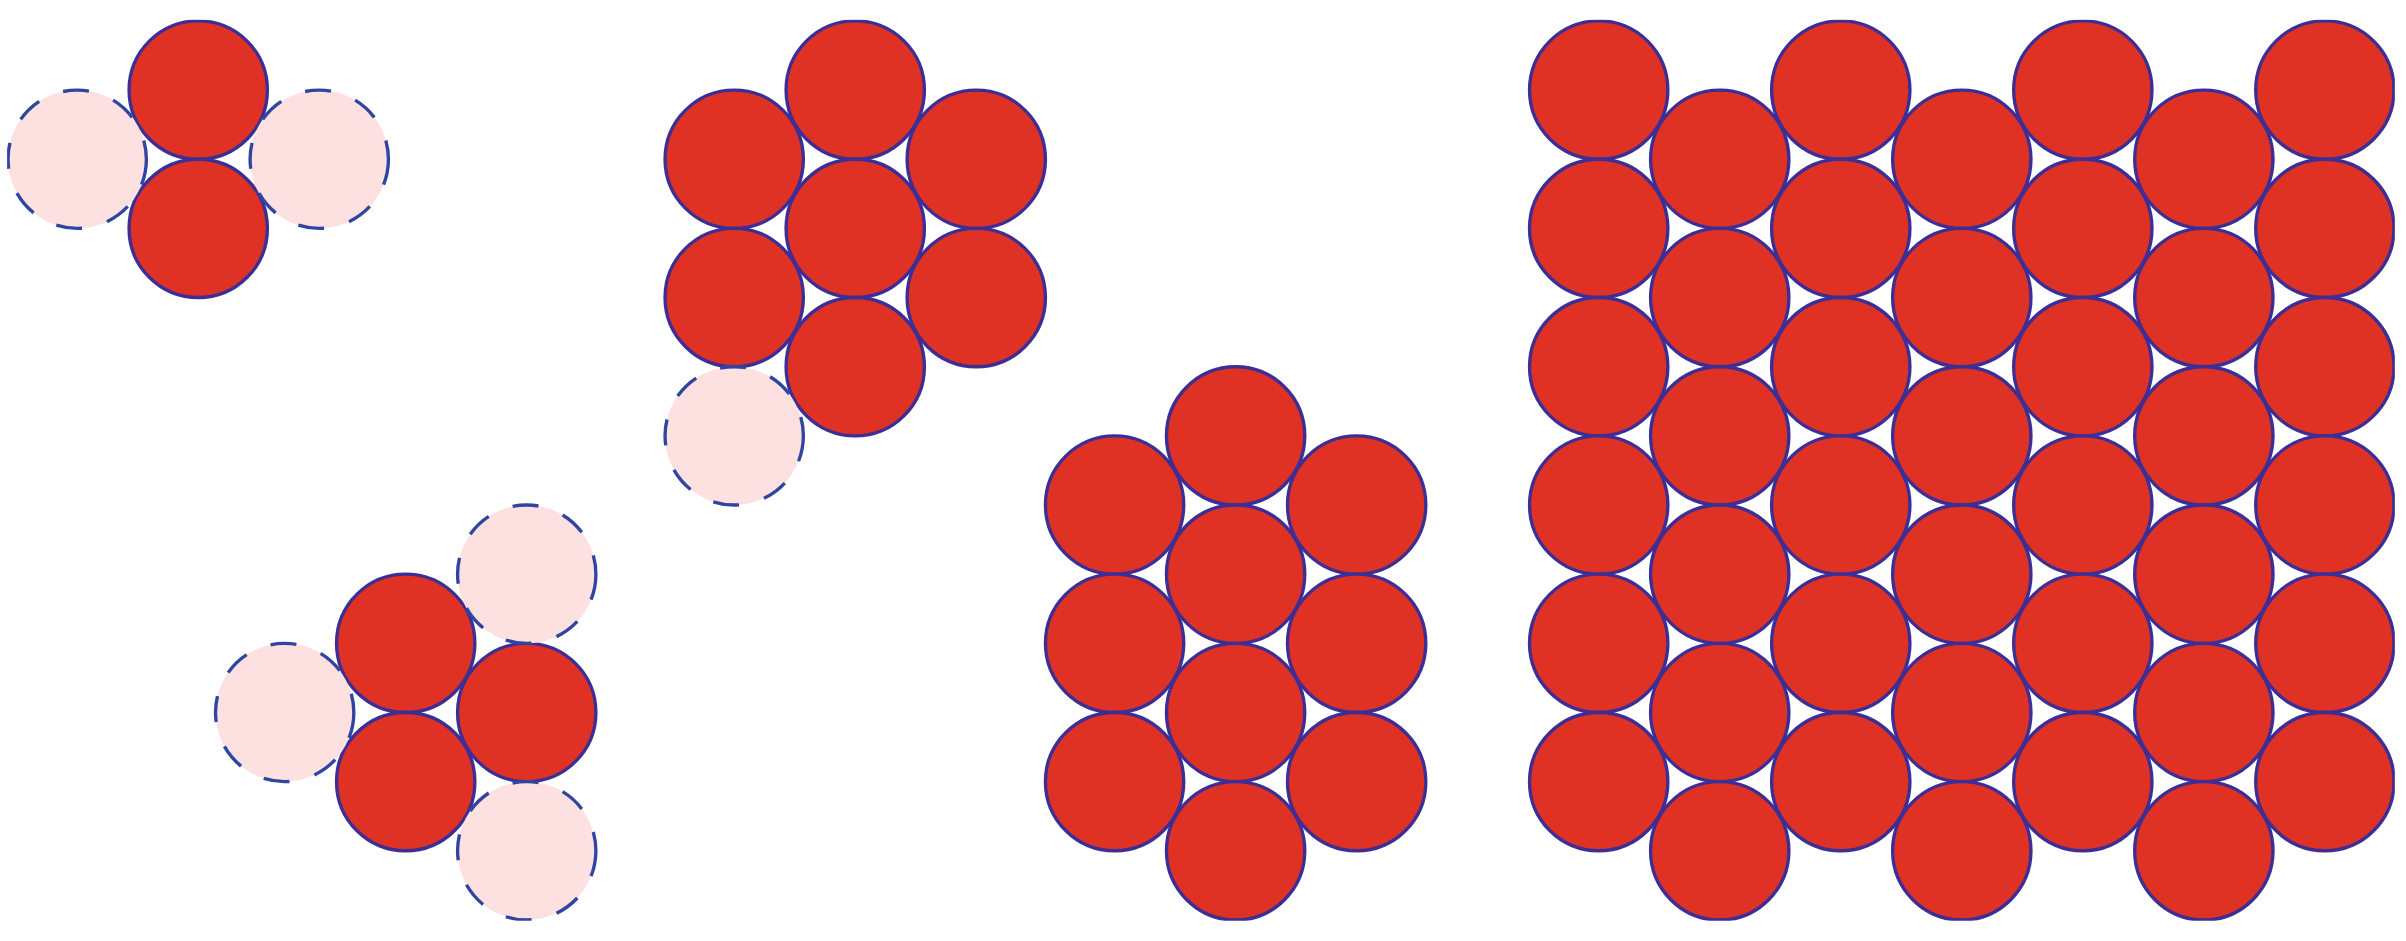
\includegraphics[width = 0.45 \textwidth]{lattice-2d.png}
	\caption{1D lattice and 2D triangular lattice of atoms.}
	\label{lat-2}
\end{figure}
\begin{figure}[!h]
	\centering
	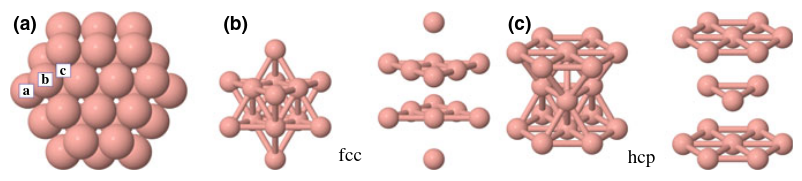
\includegraphics[width = 0.70 \textwidth]{lattice-3d.png}
	\caption{3D lattices of atoms: (a) close packing of spheres, (b) fcc lattice, (c) hcp lattice.}
	\label{lat-3}
\end{figure}

\paragraph{Difetti}

Un cristallo, a qualunque temperatura finita, ha probabilità non-nulla di formare dei \textit{difetti}, come ad esempio un atomo mancante, un atomo aggiuntivo o un'impurità (atomo di tipo diverso). In particolare, essendo il numero di atomi in un cristallo estremamente grande, la concentrazione dei difetti in un cristallo all'equilibrio a bassa temperatura va come $ \sim e^{- \beta E} $ (statistica di Boltzmann), dove $ E \sim 1 \ev $ è l'energia tipica di formazione di un difetto. Termodinamicamente, è impossibile creare un cristallo con un'estensione finita privo di difetti. \\
La piccola differenza energetica tra reticoli fcc ed hcp permette la formazione di difetti estesi (al limite anche macroscopici) come dislocazioni, stacking faults e bordi di grano (vedere Figg. \ref{def-disl}-\ref{def-st-gr}). Una dislocazione avvience quando un layer a cui manca un atomo si collega ad un layer completo: queste configurazioni sono metastabili, e con un'energia finita, a temperatura sufficientemente elevata, è possibile spostare questi difetti all'interno del cristallo. Una stacking fault avviene invece quando si interrompe e viene modificata l'alternanza regolare dei layer, mentre un bordo di grano si verifica quando si sviluppa un cristallo a partire da due punti di duplicazione diversi e con orientazioni diverse, andando a creare un'interfaccia disordinata quando queste orientazioni si incontrano.

\begin{figure}[!h]
	\centering
	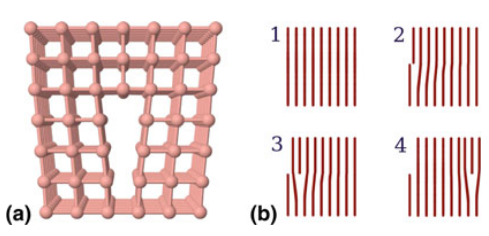
\includegraphics[width = 0.50 \textwidth]{def-disl.png}
	\caption{Dislocation in an sc lattice.}
	\label{def-disl}
\end{figure}
\begin{figure}[!h]
	\centering
	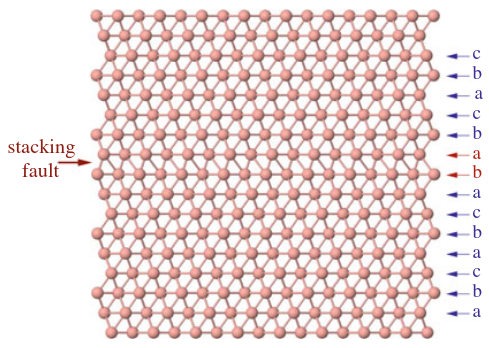
\includegraphics[width = 0.40 \textwidth]{def-st.png}
	\qquad \qquad
	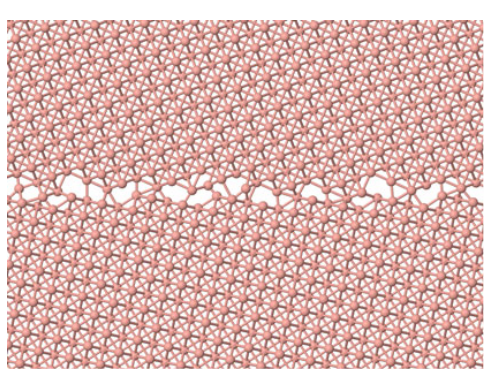
\includegraphics[width = 0.40 \textwidth]{def-gr.png}
	\caption{Stacking fault and grain boundary in an fcc lattice.}
	\label{def-st-gr}
\end{figure}

\subsection{Reticoli cristallini}

Una delle proprietà fondamentali di un solido cristallino è l'equivalenza di varie sue regioni di spazio: infatti, si può assumere che la maggior parte degli atomi di un cristallo si trovino sufficientemente lontani dal suo bordo e da qualsiasi difetto per essere modellato come appartenente ad un cristallo perfetto ed infinitamente esteso. \\
Un cristallo perfetto infinito è un insieme di punti che gode di simmetria traslazionale discreta.

\begin{definition}{Reticolo di Bravais}{}
	Si dice \textit{reticolo di Bravais} $ n $-dimensionale un insieme di punti in $ \R^n $ che risulta invariante per traslazioni discrete:
	\begin{equation}
		\ve{r} \mapsto \ve{r}' = \ve{r} + \ve{R}
		\ , \
		\ve{R} = k_1 \ve{a}_1 + \dots k_n \ve{a}_n
	\end{equation}
	con $ \{k_j\}_{j = 1,\dots,n} \subset \Z $ e $ \{\ve{a}_j\}_{j = 1,\dots,n} \subset \R^n $ linearmente indipendenti.
\end{definition}

I generatori $ \{\ve{a}_j\}_{j = 1,\dots,n} $ vengono detti \textit{primitivi} se sono $ \virgolette{i più piccoli possibili} $ (non univocamente definiti) e formano una cella primitiva, ovverosia il volume minimo che contiene tutti i punti traslazionalmente non-equivalenti del reticolo (a meno di traslazioni) e che, ripetuto nello spazio tramite traslazioni discrete, riproduce il reticolo. Nel caso tridimensionale, il volume della cella primitiva è $ V_c = \abs{(\ve{a}_1 \cdot \ve{a}_2) \times \ve{a}_3} $. \\
La cella primitiva contiene tutta l'informazione del reticolo (che è una ripetizione di tale cella), dunque il suo studio è fondamentale. Il problema, nel definirla, è che non c'è un univoco set di vettori primitivi.

\begin{definition}{Cella di Wigner-Seitz}{}
	Dato punto $ \ve{R} $ in un reticolo di Bravais, si definisce la \textit{cella di Wigner-Seitz} l'insieme di punti $ \ve{r} $ più vicini ad $ \ve{R} $ rispetto ad un altro punto $ \ve{R}' $ del reticolo.
\end{definition}

\begin{proposition}{}
	La cella di Wigner-Seitz è una cella primitiva.
\end{proposition}

L'introduzione della cella di Wigner-Seitz elimina l'arbitrarietà nella scelta della cella primitiva.

\begin{figure}
	\centering
	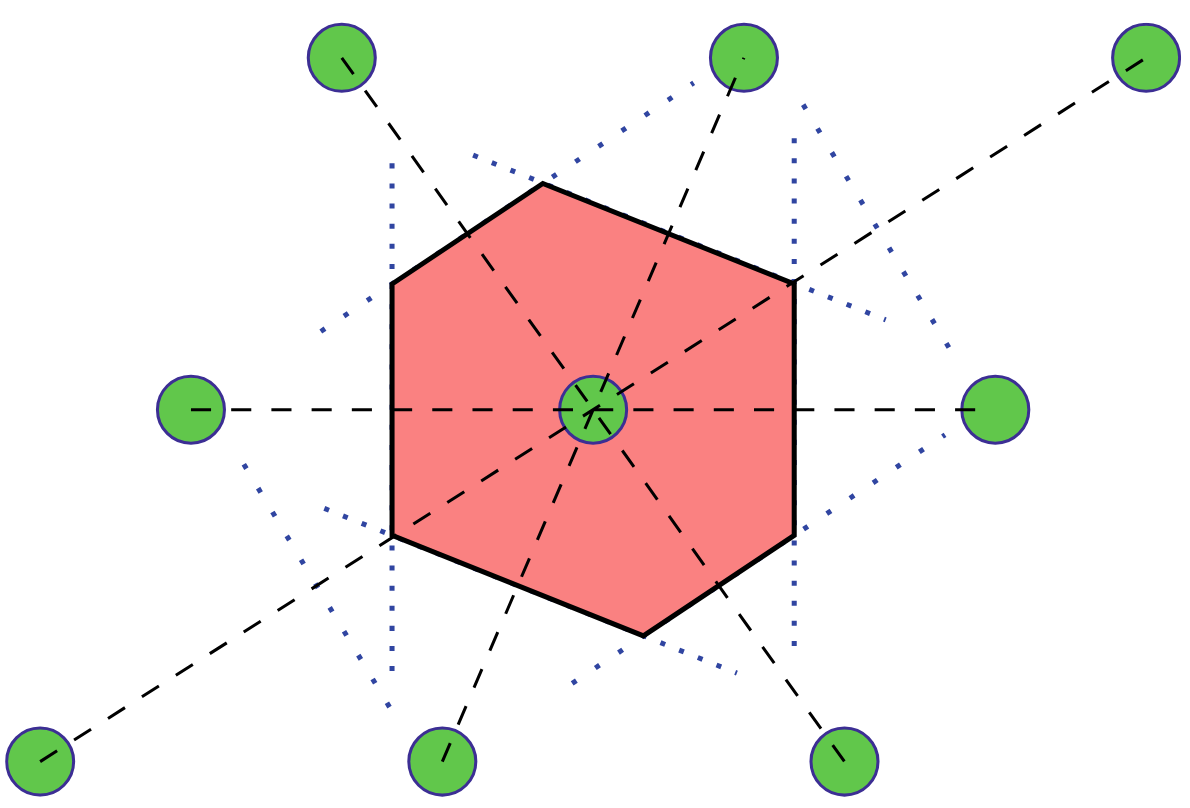
\includegraphics[width = 0.50 \textwidth]{ws-2.png}
	\caption{Wigner-Seitx cell for a 2D lattice.}
	\label{ws-2}
\end{figure}
\begin{figure}
	\centering
	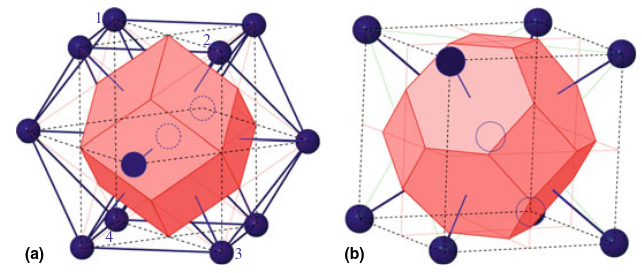
\includegraphics[width = 0.50 \textwidth]{ws-3.png}
	\quad
	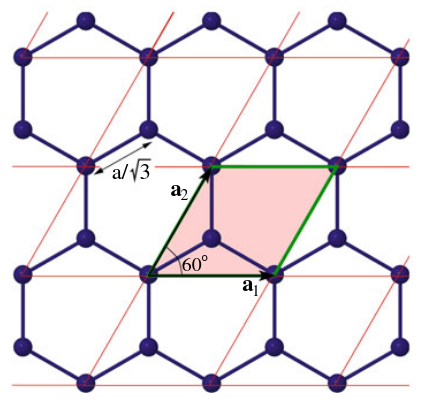
\includegraphics[width = 0.30 \textwidth]{ws-g.png}
	\caption{Wigner-Seitx cell for the fcc lattice, the bcc lattic and graphene.}
	\label{ws-3}
\end{figure}

Si noti che, in generale, una cella primitiva può contenere più di un atomo (es.: $ \ch{Na Cl} $, grafite, etc.). Infatti, un cristallo è definito da un reticolo di Bravais e da una base, ovvero un insieme di uno o più atomi ripetuti in ogni punto del retivolo. È inoltre conveniente trattare le cosiddette \textit{celle convenzionali}, ovvero insiemi di una o più celle primitive che hanno forme preferibilmente cubiche (fcc, bcc o sc), per facilitare la trattazione. Bisogna tener conto che le celle convenzionali, essendo delle super-celle, contengono informazioni ridondanti rispetto alle celle primitive.

\subsubsection{Reticolo reciproco}

Si consideri una funzione $ f : \R \rightarrow \R $ periodica con periodo $ a \in \R $, ovvero tale per cui $ f(x -na) = f(x) \,\,\forall n \in \Z $. La sua antitrasformata di Fourier è:
\begin{equation}
	f(x) = \int_\R \frac{\dd k}{\sqrt{2\pi}} e^{ikx} \tilde{f}(k)
\end{equation}
I coefficienti di Fourier $ \tilde{f}(k) $ sono nulli, eccetto quelli con lo stesso periodo di $ f(x) $, ovvero quelli con $ e^{ikx} = e^{ik(x-a)} $: ciò equivale a $ e^{-ika} = 1 $, ovvero $ k = \ell \frac{2\pi}{a} $, con $ \ell \in \Z $. Questi valori vengono convenzionalmente indicati come:
\begin{equation}
	G = \frac{2\pi}{a} \ell
\end{equation}
e forniscono le frequenze discrete, nello spazio reciproco, che costituiscono la serie di Fourier di $ f(x) $:
\begin{equation}
	f(x) = \sum_G e^{iGx} \tilde{f}(G)
	\qquad \qquad
	\tilde{f}(G) = \frac{1}{a} \int_0^a \dd x\, e^{-i G x} f(x)
\end{equation}
I punti $ G $ nello spazio reciproco formano un reticolo, detto \textit{reticolo reciproco}, legato al reticolo nello spazio diretto da:
\begin{equation}
	e^{i G R} = e^{i 2\pi n \ell} = 1
\end{equation}
dove $ R = na $ sono le traslazioni del reticolo diretto. Si trova quindi $ \ell = \frac{1}{n} $. \\
Queste definizioni sono generalizzabili al caso 3D, in cui $ \ve{R} = n_1 \ve{a}_1 + n_2 \ve{a}_2 + n_3 \ve{a}_3 $. In questo caso, la condizione di reciprocità diventa:
\begin{equation}
	e^{i \ve{G} \cdot \ve{R}} = 1
	\label{eq:rec-ret}
\end{equation}
In 3D si trova che:
\begin{equation}
	\ve{G} = \ell_1 \ve{b}_1 + \ell_2 \ve{b}_2 + \ell_3 \ve{b}_3
\end{equation}
con $ \ell_1, \ell_2, \ell_3 \in \Z $ e:
\begin{equation}
	\ve{b}_1 = \frac{2\pi}{V_c} \ve{a}_2 \times \ve{a}_3
	\qquad
	\ve{b}_1 = \frac{2\pi}{V_c} \ve{a}_2 \times \ve{a}_3
	\qquad
	\ve{b}_1 = \frac{2\pi}{V_c} \ve{a}_2 \times \ve{a}_3
\end{equation}
Si noti che $ \ve{a}_i \cdot \ve{b}_j = 2\pi $, dunque $ \ve{G} \cdot \ve{R} = 2\pi (n_1 \ell_1 + n_2 \ell_2 + n_3 \ell_3) $. La serie di Fourier in 3D diventa:
\begin{equation}
	f(\ve{x}) = \sum_\ve{G} e^{i \ve{G} \cdot \ve{x}} \tilde{f}(\ve{G})
	\qquad \qquad
	\tilde{f}(\ve{G}) = \frac{1}{V_c} \int_{V_c} \dd^3x\, e^{-i \ve{G} \cdot \ve{x}} f(\ve{x})
\end{equation}
Il volume della cella primitiva del reticolo reciproco è $ \tilde{V}_c = (\ve{b}_1 \times \ve{b}_2) \cdot \ve{b}_3 = \frac{(2\pi)^3}{V_c} $: questa viene detta \textit{prima zona di Brillouin} (BZ).

\begin{example}{Reticoli reciproci}{}
	Il reticolo reciproco di un fcc con cubo di lato $ a $ è un bcc con cubo di lato $ 4\pi/a $ e viceversa, mentre il reticolo reciproco di un sc con cubo di lato $ a $ è un sc con cubo di lato $ 2\pi/a $.
\end{example}

Ciascun $ \ve{G} $ nel reticolo reciproco definisce un'onda piana $ e^{i \ve{G} \cdot \ve{x}} $ (nello spazio diretto) con la stessa periodicità del reticolo diretto. Se si considerano i fronti d'onda fissati, per esempio, da $ e^{i \ve{G} \cdot \ve{x}} = 1 $, questi formano una famiglia di piani paralleli tra loro e perpendicolari a $ \ve{G} $ (che ne dà la direzione di propagazione), separati tra loro da una distanza $ \lambda = 2\pi / \abs{\ve{G}} $. \\
Alcuni di questi piani passano per punti del reticolo reciproco; in particolare, tutti questi piani passano per punti del reticolo reciproco se gli indici interi $ (\ell_1 \, \ell_2 \, \ell_3) $ che definiscono $ \ve{G} $ non hanno divisori non-banali comuni: questi vengono detti \textit{indici di Miller} della famiglia di piani considerata. Se invece $ \ve{G} $ è determinato da $ (n\ell_1 \, n\ell_2 \, n\ell_3) $, con $ n \in \Z - \{0\} $, allora soltanto un piano ogni $ n $ passerà per punti del reticolo diretto. \\
Si dimostra che gli indici di Miller sono proporzionali ai reciproci delle intercette dei piani con le direzioni dei vettori primitivi del reticolo diretto.

\subsection{Diffrazione}

La diffrazione da sonde wave-like è il principale mezzo d'indagine della struttura interna dei cristalli, data la loro natura periodica. La lunghezza d'onda di tali sonde deve essere comparabile con la tipica dimensione delle celle primarie del cristallo, tipicamente $ \sim 0.1 - 1 \,\text{nm} $: ciò corrisponde ad elettroni con energia cinetica $ \sim 1.5 - 150 \ev $, raggi X nel range $ \sim 1 - 10 \kev $ o neutroni con energia cinetica $ \sim 1 - 100 \,\text{meV} $. Gli elettroni interagiscono fortemente con la materia, dunque sono sensibili solo agli strati superficiali del cristallo; se si escludono energie risonanti con stati di core atomici, i raggi X riescono a penetrare anche per migliaia di celle primarie, andando a sondare le proprietà di bulk del cristallo; infine i neutroni, interagendo solo coi nuclei (dunque con sezione d'urto molto piccola), riescono a penetrare anche nell'ordine del centimetro. \\
Si assuma che il raggio incidente sia prodotto da una sorgente lontana, così da avere un vettore d'onda $ \ve{k} $ ben definito (con $ \abs{\ve{k}} = 2\pi/\lambda) $, e che il raggio uscente sia rilevato da un detector lontano, così da rilevare un $ \ve{k}' $ ben definito. Nell'ipotesi di scattering elastico, si ha $ \abs{k} = \abs{k}' $ (ovvero $ \lambda = \lambda' $) e si definisce il vettore d'onda trasferito come $ \ve{q} \equiv \ve{k}' - \ve{k} $. Dato che ogni volume infinitesimo $ \dd^3r $ scattera il raggio incidente in porporzione al numero di scatterers in esso presente $ n(\ve{r}) \dd^3r $ (con $ n(\ve{r}) $ densità numerica), la probabilità totale di osservare lo scattering $ \ve{k} \rightarrow \ve{k}' $ è (ricordando che sono onde):
\begin{equation*}
	P_{\ve{k} \rightarrow \ve{k}'} \propto \abs{\int_V \dd^3r\, n(\ve{r}) e^{-i \ve{k}' \cdot \ve{r}} e^{i \ve{k} \cdot \ve{r}}}^2 = \abs{\int_V \dd^3r\, n(\ve{r}) e^{-i \ve{q} \cdot \ve{r}}}^2 \propto \abs{\tilde{n}(\ve{q})}^2
\end{equation*}
dove $ \tilde{n}(\ve{q}) $ è la trasformata di Fourier della densità numerica di scatterers $ n(\ve{r}) $ (a seconda della sonda, sarà la densità numerica di nuclei $ n_\text{nucl}(\ve{r}) $ se la sonda è composta da neutroni, mentre sarà quella di elettroni $ n_\text{el}(\ve{r}) $ se composta da raggi X). Si trova quindi che l'intensità del fascio scatterato va come:
\begin{equation}
	I(\ve{q}) \propto \abs{\tilde{n}(\ve{q})}^2
\end{equation}
La densità numerica di un solo atomo è una $ \delta $ di Dirac, ed infatti l'intesità da scatter neutronico di un solo atomo è essenzialmente indipendente da $ \ve{q} $, come si vede in Fig. \ref{diffr}. \\
Se invece si considerano due atomi, si avrà inferferenza tra i raggi scatterati dai due centri di diffusione. Considerando le posizioni $ \ve{R}_1 , \ve{R}_2 $ dei due atomi, si ha qualitativamente che:
\begin{equation*}
	\begin{split}
		\abs{\tilde{n}(\ve{q})}^2
		& \propto \abs{e^{-i \ve{R}_1 \cdot \ve{q}} + e^{-i \ve{R}_2 \cdot \ve{q}}}^2 = \abs{\exp \left( -i \frac{\ve{R}_1 + \ve{R}_2}{2} \cdot \ve{q} \right) 2 \cos \left( \frac{\ve{R}_1 - \ve{R}_2}{2} \cdot \ve{q} \right)}^2 \\
		& = 2 \left[ 1 + \cos \left( (\ve{R}_1 - \ve{R}_2) \cdot \ve{q} \right) \right] = 2 \left[ 1 + \cos (a q_x) \right]
	\end{split}
\end{equation*}
dove si è supposto che $ \ve{R}_1 - \ve{R}_2 = a \hat{\ve{e}}_x $ e $ \hat{\ve{e}}_x \cdot \ve{q} = q_x $. Si vede dunque che la condizione di interferenza costruttiva (così da avere picchi di diffrazione) è:
\begin{equation*}
	aq_x = 2\pi \ell
	\qquad \Rightarrow \qquad
	q_x = \frac{2\pi}{a} \ell
\end{equation*}
Considerando un reticolo 3D di $ N $ atomi, quindi, la trasformata della densità numerica va come:
\begin{equation*}
\abs{\tilde{n}(\ve{q})}^2 \propto \abs{\sum_{j = 1}^N e^{-i \ve{R}_j \cdot \ve{q}}}^2
\end{equation*}
La condizione d'interferenza costruttiva è quindi:
\begin{equation}
	e^{-i \ve{R} \cdot \ve{q}} = 1 \quad \forall \ve{R} \in \text{reticolo}
	\label{eq:cond-int-cos}
\end{equation}
Questa non è altro che l'Eq. \ref{eq:rec-ret}: si trova quindi che i picchi di diffrazione, detti \textit{picchi di Bragg}, si hanno per vettori d'onda trasferiti appartenente al reticolo recièroco, ovvero per $ \ve{q} = \ve{G} $. Si noti che può accadere che la condizione \ref{eq:cond-int-cos} può essere verificata anche solo per alcuni $ \ve{R} \in \text{reticolo} $: in tal caso, si hanno dei picchi di diffrazione secondari, la cui intensità decresce rapidamente all'aumentare del numero di atomi nel reticolo (si veda Fig. \ref{diffr}).

\begin{figure}
	\centering
	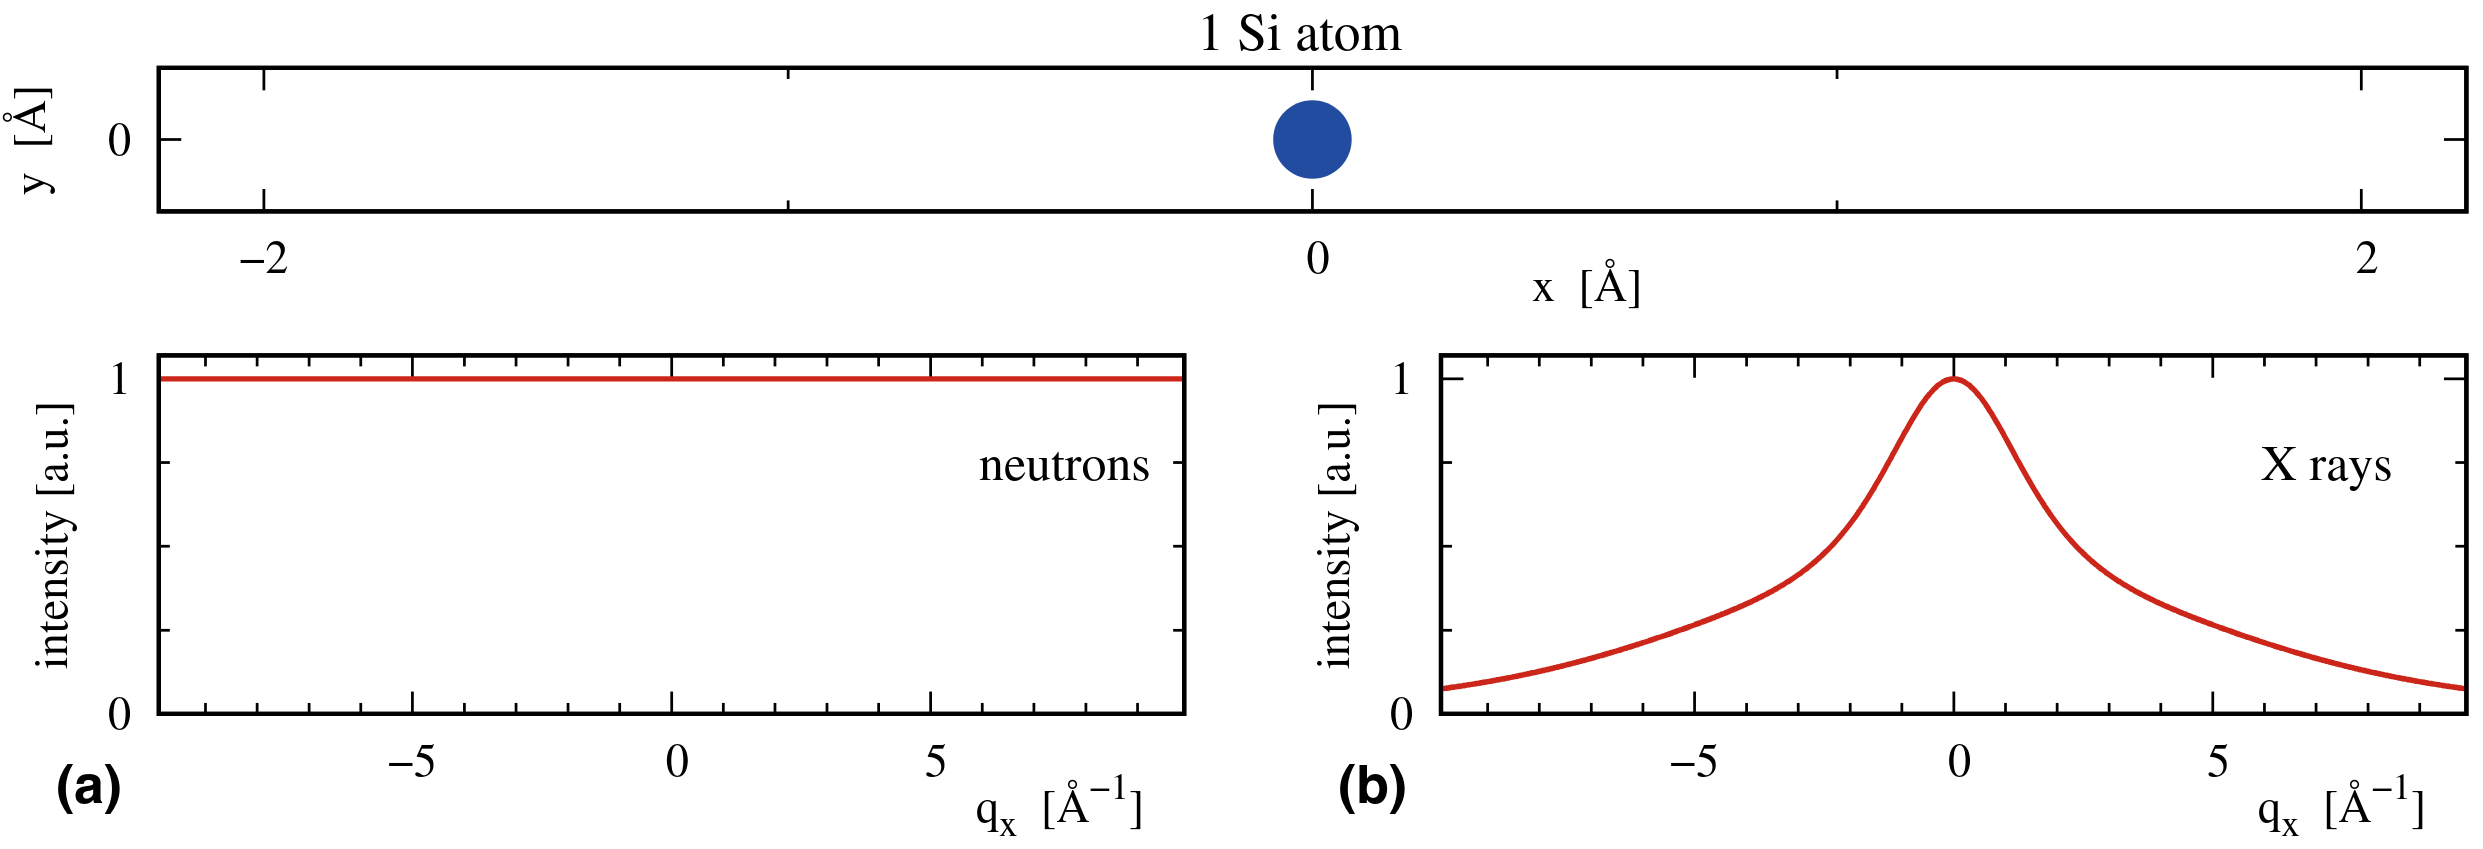
\includegraphics[width = 0.70 \textwidth]{diffr-1.png}
	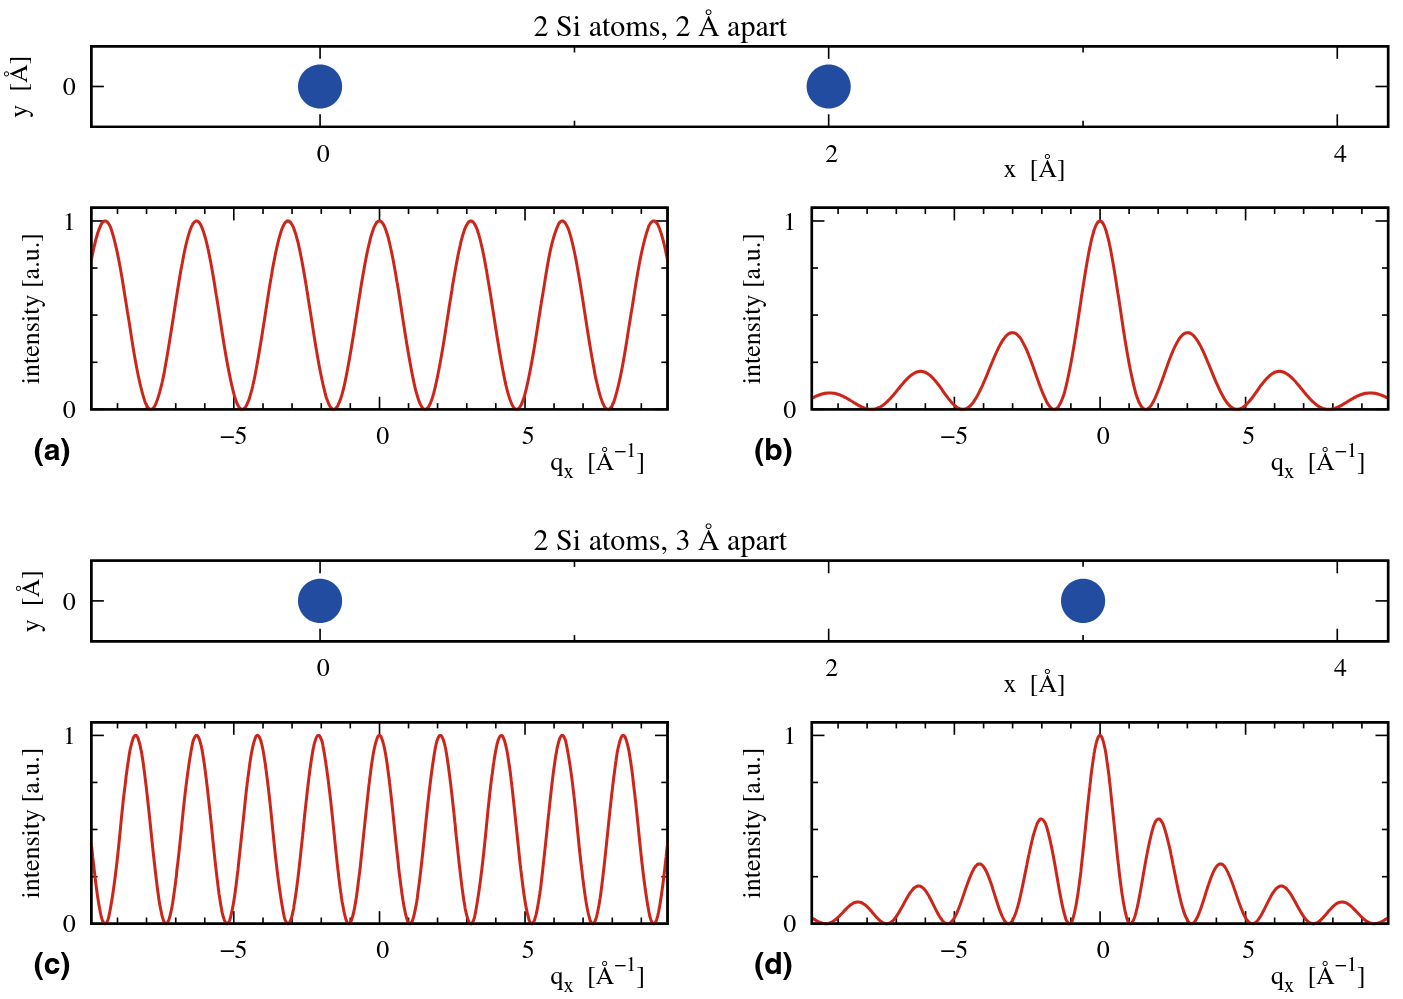
\includegraphics[width = 0.70 \textwidth]{diffr-2.png}
	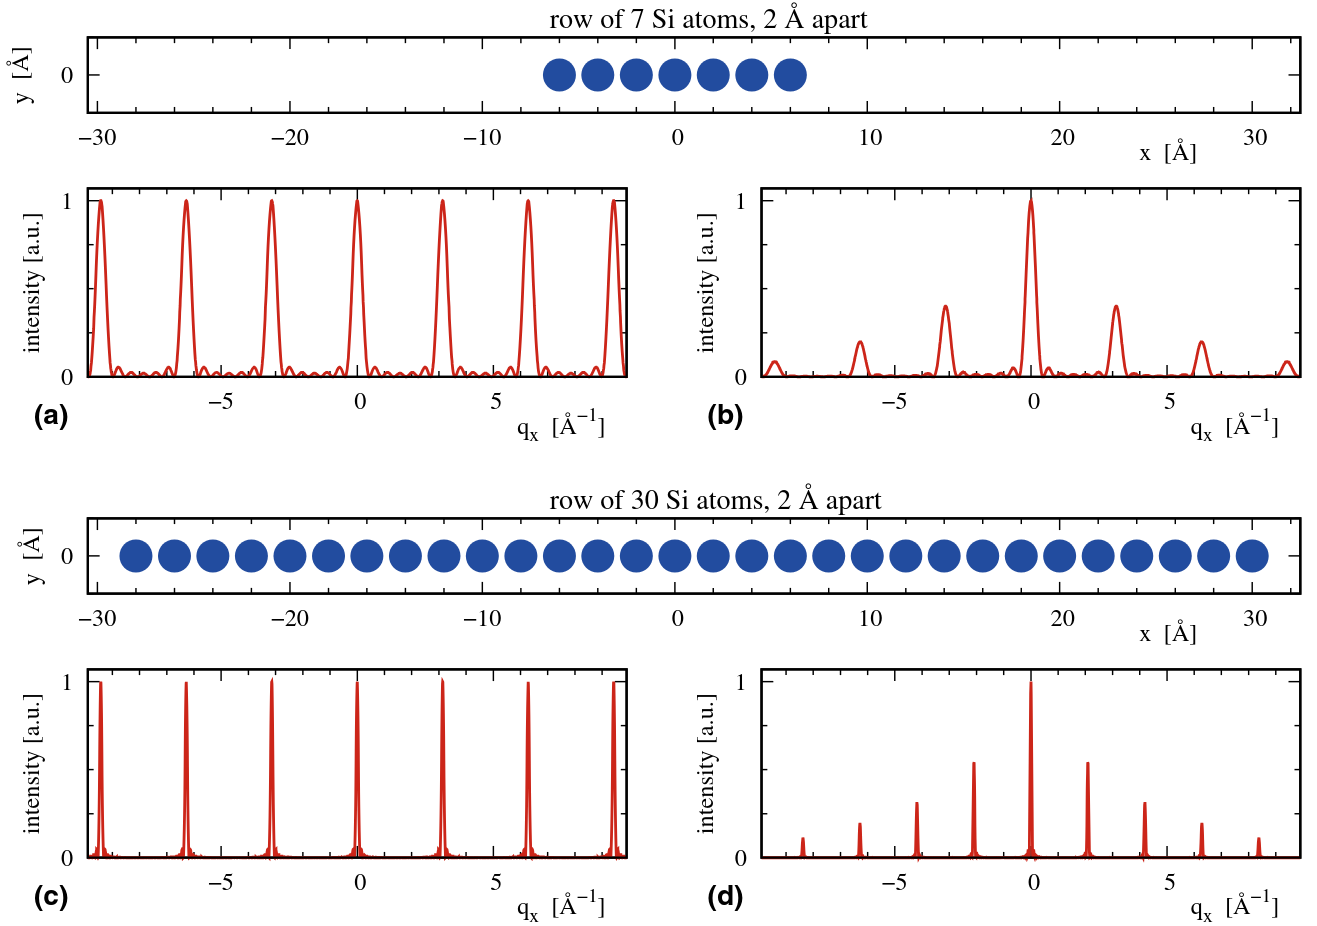
\includegraphics[width = 0.70 \textwidth]{diffr-3.png}
	\caption{Diffraction patterns of various 1D chains of $ \ch{Si} $ atoms.}
	\label{diffr}
\end{figure}

\subsubsection{Fattori di forma}

Raggi X che scatterano su un singolo atomo ne sondano la distribuzione di densità elettronica $ n_\text{at}(\ve{r}) $, tramite il \textit{fattore di forma atomico} $ f_\text{at}(\ve{q}) = \tilde{n}_\text{at}(\ve{q}) $: questo ha una caratteristica forma a campana con $ f_\text{at}(\ve{0}) $ pari al quadrato del numero di elettroni. \\
Per $ Z \gg 1 $, gli elettroni di core scatterano di più i raggi X rispetto ai meno numerosi elettroni di valenza, così che, per un insieme di atomi, la distribuzione elettronica vista dai raggi X possa essere approssimata come la somma delle individuali distribuzioni atomiche:
\begin{equation}
	n_\text{el}(\ve{r}) = \sum_\ve{R} n_\text{at}(\ve{r} - \ve{R})
\end{equation}
La presenza di legami chimici deforma soltanto i relativamente pochi elettroni di valenza, così che tale approssimazione dia un buon accordo sperimentale. Calcolando la trasformata di Fourier:
\begin{equation*}
	\begin{split}
		\tilde{n}_\text{el}(\ve{q})
		& = \sum_\ve{R} \int \dd^3r\, n_\text{at}(\ve{r} - \ve{R}) e^{-i \ve{q} \cdot \ve{r}} = \sum_\ve{R} \int \dd^3r'\, n_\text{at}(\ve{r}') e^{-i \ve{q} \cdot (\ve{r}' + \ve{R})} \\
		& = \sum_\ve{R} e^{-i \ve{q} \cdot \ve{R}} \int \dd^3r\, n_\text{at}(\ve{r}) e^{-i \ve{q} \cdot \ve{r}} \equiv \tilde{n}_\text{ret}(\ve{q}) f_\text{at}(\ve{q})
	\end{split}
\end{equation*}
Si hanno dunque due contributi moltiplicativi (si ricordi che un prodotto nello spazio reciproco è una convoluzione nello spazio reale): $ \tilde{n}_\text{ret}(\ve{q}) $, che descrive lo scattering da oggetti puntiformi posti nei nodi del reticolo di Bravais, ed $ f_\text{at}(\ve{q}) $, che descrive lo scattering dagli atomi singoli. Dato che $ n_\text{nuc}(\ve{r}) \propto n_\text{ret}(\ve{r}) $, si trova una relazione tra l'intensità della diffrazione da raggi X e quella da neutroni:
\begin{equation}
	I_\text{X}(\ve{q}) \propto \abs{f_\text{at}(\ve{q})}^2 \abs{\tilde{n}_\text{nuc}(\ve{q})}^2 \propto \abs{f_\text{at}(\ve{q})}^2 I_\text{n}(\ve{q})
\end{equation}
Questa relazione di proporzionalità è confermata in Fig. \ref{diffr}: i raggi X scatterano nelle stesse direzioni e con le stesse lunghezze d'onda dei neutroni, ma l'intensità dei picchi è modulata da $ \abs{f_\text{at}(\ve{q})}^2 $. \\
Se si considerano cristalli poliatomici la cui cella primitiva contiene $ n_d $ atomi, la derivazione rimane invariata, sommando anche su questi atomi:
\begin{equation}
	n_\text{el}(\ve{r}) = \sum_\ve{R} \sum_{j = 1}^{n_d} n_{\text{at},j}(\ve{r} - \ve{d}_j - \ve{R})
\end{equation}
Si trova così che il fattore di forma atomico va sostituito con un \textit{fattore di struttura}:
\begin{equation}
	S(\ve{q}) = \sum_{j = 1}^{n_d} e^{-i \ve{q} \cdot \ve{d}_j} f_{\text{at},j}(\ve{q})
\end{equation}
rappresentante la trasformata di Fourier della distribuzione elettronica degli $ n_d $ atomi nella cella primaria. Nello scattering di neutroni, gli $ f_{\text{at},j}(\ve{q}) $ sono sostituiti da ampiezze di scattering neutronico indipendenti da $ \ve{q} $. Si trova dunque che, posto $ \abs{f_\text{at}(\ve{q})}^2 \mapsto \abs{S(\ve{q})}^2 $, la forma di $ I(\ve{q}) $ rimane pressoché invariata: ciò significa che il pattern di diffrazione è sostanzialmente indipendente dal numero di atomi nella cella primaria, ma è determinato dal reticolo di Bravais del cristallo; gli atomi nella cella primaria vanno soltanto a modificare moltiplicativamente l'intensità, senza modificarne la forma.

\subsubsection{Scattering di Bragg}

Come si è visto, la condizione per cui si hanno picchi di diffrazione è $ \ve{q} = \ve{G} $. In aggiunta a ciò, per avere scattering elastico è necessario che $ \abs{\ve{k}} = \abs{\ve{k}'} $, ovvero:
\begin{equation}
	\abs{\ve{k}} = \abs{\ve{k} + \ve{G}}
	\label{eq:bragg-diffr}
\end{equation}
Questa condizione corrisponde geometricamente ad una sfera nello spazio reciproco, rappresentata dalla \textit{costruzione di Ewald} (Fig. \ref{diffr-e}): se questa sfera interseca più punti del reticolo reciproco, allora è possibile avere interferenza costruttiva e dunque diffrazione.
Elevando al quadrato si trova $ 2 \ve{k} \cdot \ve{G} + \abs{\ve{G}}^2 = 0 $, ovvero:
\begin{equation}
	\ve{k} \cdot \hat{\ve{G}} = - \frac{\abs{\ve{G}}}{2}
\end{equation}

\begin{figure}
	\centering
	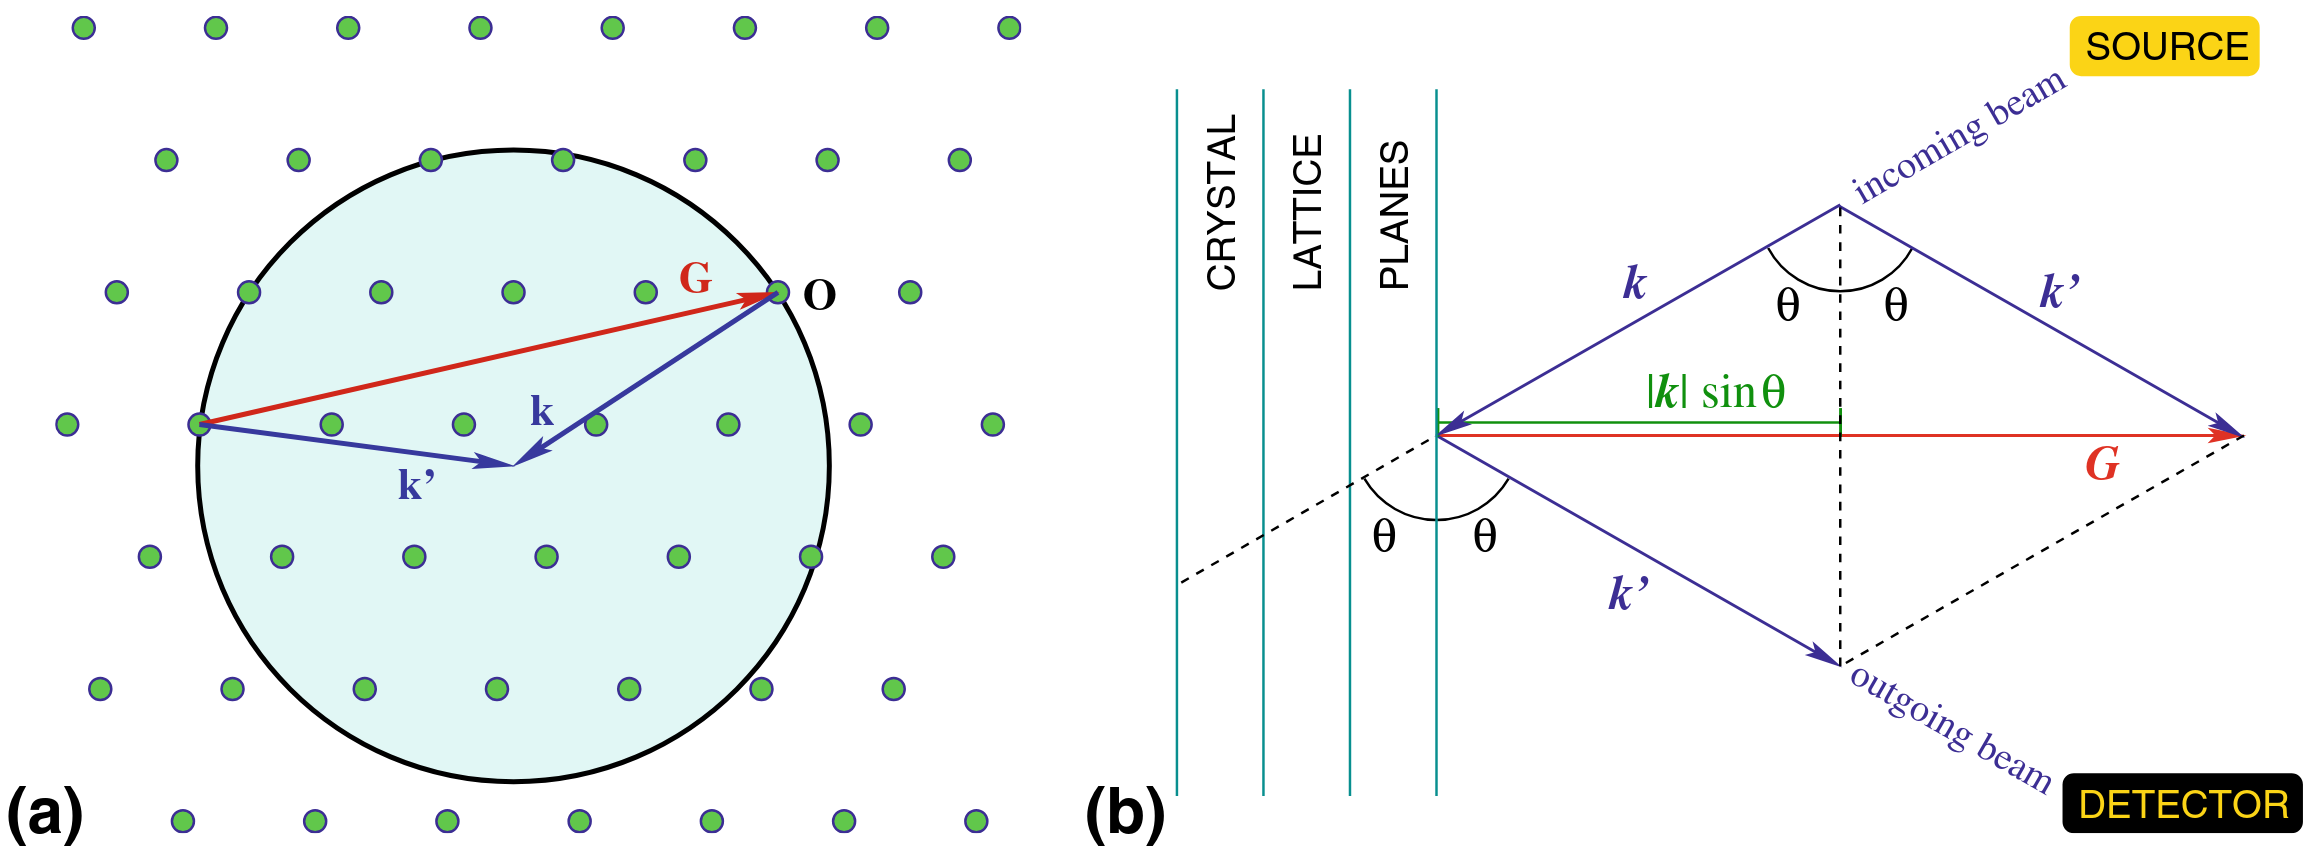
\includegraphics[width = 0.70 \textwidth]{diffr-e.png}
	\caption{Ewald construction.}
	\label{diffr-e}
\end{figure}

Come si vede in Fig. \ref{diffr-e}, vale la relazione $ \ve{k} \cdot \hat{\ve{G}} = - \sin \theta $, dove l'angolo di scattering tra $ \ve{k} $ e $ \ve{k}' $ è $ 2\theta $. Essendo i piani nel reticolo associati a $ \ve{G} $ separati da una distanza $ d = n \frac{2\pi}{\abs{\ve{G}}} $, dove $ n $ è il massimo comun divisore degli indici di Miller di $ \ve{G} $, ed valendo la relazione $ \abs{\ve{k}} = \frac{2\pi}{\lambda} $, dove $ \lambda $ è la lunghezzaq d'onda della radiazione incidente, si trova la \textit{condizione di Bragg} per la diffrazione:
\begin{equation}
	2 d \sin \theta = n \lambda
\end{equation}
Secondo questa equazione (e come confermato in Fig. \ref{diffr-e}), non avviene diffrazione per $ \lambda > 2d $. Nella pratica, per generare dei raggi diffratti da un singolo cristallo, si muove il reticolo reciproco rispetto alla sfera di Ewald fino a quando non ci sono almeno due punti che la intersecano: per fare ciò, o si varia la lunghezza d'onda incidente, andando a modificare il raggio della sfera di Ewald, o si ruota il cristallo (dato che il reticolo reciproco ruota della stessa quantità di quello reale). \\
Solitamente si studiano le \textit{polveri}, ovvero insiemi di microcristalli ruotati randomicamente nello spazio: la distribuzione uniforme di orientazioni equivale ad una media sulle possibili rotazioni del reticolo reciproco. Di conseguenza, nella costruzione della sfera di Ewald per una polvere, si possono considerare non solo i punti che intersecano la sfera, ma anche le intersezioni delle possibili rotazioni di tale sfera, ottenendo una maggiore possibilità di ottenere un pattern di diffrazione. \\
Infine, si noti che difetti e dimensione finita del cristallo pongono i picchi di Bragg su un background continuo diffuso: all'aumentare del disordine l'intensità del background cresce, fino a quando non sono più presenti picchi di Bragg (solidi amorfi, liquidi).

\section{Elettroni}

All'interno dei solidi, gli elettroni si muovo secondo l'equazione elettronica Eq. \ref{eq:mol-el-eq}: perciò, è possibile definire un potenziale adiabatico (Eq. \ref{eq:ad-pot}) che descrive il moto dei nuclei (Eq. \ref{eq:mol-nucl-eq}).

\subsection{Elettroni nei cristalli}

Nei solidi cristallini a basse temperature, il potenziale adiabatico la configurazione atomica in un intorno del minimo di potenziale, ovverosia mantiene i nuclei fissi nelle posizioni reticolari. Invocando la separazione adiabatica, dunque, si assume che i nuclei abbiano energia cinetica trascurabile e siano fissi nel reticolo, così da ridurre il problema a quello elettronico. \\
Innanzitutto, data la simmetria reticolare del cristallo, si ha che l'Hamiltoniana elettronica è invariante per le traslazioni discrete del reticolo:
\begin{equation}
	[\hat{\mathcal{H}} , \hat{T}_\ve{R}] = 0 \quad \forall \ve{R} \in \text{reticolo}
\end{equation}
Di conseguenza, le autofunzioni $ \phi(\ve{r}) $ dell'Hamiltoniana devono soddisfarre:
\begin{equation}
	\hat{T}_\ve{R} \phi(\ve{r}) = \alpha_\ve{R} \phi(\ve{r})
\end{equation}
con $ \alpha_\ve{R} \in \C $. Essendo il cristallo un sistema periodico, si deve poter applicare $ \hat{T}_\ve{R} $ un numero arbitrario di volte: se $ \abs{\alpha_\ve{R}} < 1 $ la densità di probabilità tende ad annullarsi, all'aumentare del numero di $ \hat{T}_\ve{R} $ applicati, mentre se $ \abs{\alpha_\ve{R}} > 1 $ tende a divergere. L'unica possibilità, dunque, è:
\begin{equation*}
	\abs{\alpha_\ve{R}} = 1
	\qquad \Rightarrow \qquad
	\alpha_\ve{R} = e^{-i \varphi_\ve{R}}
\end{equation*}
Un'altra proprietà che $ \hat{T}_\ve{R} $ deve soddisfare è la legge compositiva del gruppo:
\begin{equation*}
	\hat{T}_{\ve{R}_1} \hat{T}_{\ve{R}_2} = \hat{T}_{\ve{R}_1 + \ve{R}_2}
	\qquad \Rightarrow \qquad
	\varphi_{\ve{R}_1} \varphi_{\ve{R}_2} = \varphi_{\ve{R}_1 + \ve{R}_2}
\end{equation*}
Si può prendere WLOG $ \varphi_\ve{R} = \ve{q} \cdot \ve{R} $, con $ \ve{q} \in \R $, ma si noti che esso non è univocamente determinato: infatti, dall'Eq. \ref{eq:rec-ret}, si ha che:
\begin{equation*}
	e^{-i \ve{q} \cdot \ve{R}} = e^{-i (\ve{q} + \ve{G}) \cdot \ve{R}} \quad \forall \ve{G} \in \text{reticolo reciproco}
\end{equation*}
Ciò significa che $ \ve{q} $ è definito a meno di un qualsiasi vettore $ \ve{G} $ del reticolo reciproco. Questo permette di ridurre $ \ve{q} $ ad un vettore $ \ve{k} $ nella prima BZ scegliendo un opportuno $ \ve{G} $. La trattazione dell'intero cristallo è così ridotta alla sola prima BZ, e l'operatore traslazione agisce come:
\begin{equation}
	\hat{T}_\ve{R} \phi(\ve{r}) = \phi(\ve{r} - \ve{R}) = e^{-i \ve{k} \cdot \ve{R}} \phi(\ve{r})
	\label{eq:trasl-op}
\end{equation}

\begin{theorem}{Teorema di Bloch}{}
	In un reticolo cristallino, ogni funzione d'onda elettronica è un'onda piana modulata da una funzione periodica:
	\begin{equation}
		\phi(\ve{r}) = e^{i \ve{k} \cdot \ve{r}} u_\ve{k}(\ve{r})
		\qquad \qquad
		u_\ve{k}(\ve{r}) = u_\ve{k}(\ve{r} - \ve{R})
		\label{eq:bloch-th}
	\end{equation}

	\tcblower

	\begin{proof}
		Dall'Eq. \ref{eq:trasl-op}:
		\begin{equation*}
			\begin{split}
				\phi(\ve{r} - \ve{R})
				& = e^{-i \ve{k} \cdot \ve{R}} \phi(\ve{r}) \\
				& = e^{i \ve{k} \cdot (\ve{r} - \ve{R})} u_\ve{k}(\ve{r} - \ve{R}) = e^{-i \ve{k} \cdot \ve{R}} e^{i \ve{k} \cdot \ve{r}} u_\ve{k}(\ve{r}) = e^{-i \ve{k} \cdot \ve{R}} \phi(\ve{r})
			\end{split}
		\end{equation*}
	\end{proof}
\end{theorem}

È possibile esprimere la funzione periodica $ u_\ve{k}(\ve{r}) $ in serie di Fourier discreta:
\begin{equation}
	u_\ve{k}(\ve{r}) = \sum_\ve{G} c_{\ve{G},\ve{k}} e^{i \ve{G} \cdot \ve{r}}
	\qquad \Rightarrow \qquad
	\phi(\ve{r}) = \sum_\ve{G} c_{\ve{G},\ve{k}} e^{i (\ve{G} + \ve{k}) \cdot \ve{r}}
\end{equation}

\begin{proposition}{Equazione elettronica}{}
	L'equazione elettronica in un cristallo è:
	\begin{equation}
		\left[ -\frac{\hbar^2}{2m_e} (\nabla + i\ve{k})^2 + V_\text{eff}(\ve{r}) \right] u_{j,\ve{k}}(\ve{r}) = E_{j,\ve{k}} u_{j,\ve{k}}(\ve{r})
		\label{eq:lat-el-eq}
	\end{equation}
	con $ V_\text{eff} \equiv V_{ee} + V_{ne} $ nella prima BZ.

	\tcblower

	\begin{proof}
		Dall'Eqq. \ref{eq:mol-el-eq}-\ref{eq:bloch-th}, l'equazione elettronica può essere scritta nella prima BZ come:
		\begin{equation*}
			\left[ -\frac{\hbar^2}{2m_e} \nabla^2 + V_\text{eff}(\ve{r}) \right] e^{i \ve{k} \cdot \ve{r}} u_{j,\ve{k}}(\ve{r}) = E_{j,\ve{k}} e^{i \ve{k} \cdot \ve{r}} u_{j,\ve{k}}(\ve{r})
		\end{equation*}
		Il termine cinetico viene riscritto come:
		\begin{equation*}
			\begin{split}
				\nabla^2 \left[ e^{i \ve{k} \cdot \ve{r}} u_{j,\ve{k}}(\ve{r}) \right]
				& = \nabla \cdot \left[ e^{i \ve{k} \cdot \ve{r}} \nabla u_{j,\ve{k}}(\ve{r}) + i \ve{k} e^{i \ve{k} \cdot \ve{r}} u_{j,\ve{k}}(\ve{r}) \right] \\
				& = e^{i \ve{k} \cdot \ve{r}} \nabla^2 u_{j,\ve{k}}(\ve{r}) + 2 e^{i \ve{k} \cdot \ve{r}} i \ve{k} \cdot \nabla u_{j,\ve{k}}(\ve{r}) - \abs{\ve{k}}^2 e^{i \ve{k} \cdot \ve{r}} u_{j,\ve{k}}(\ve{r}) \\
				& = e^{i \ve{k} \cdot \ve{r}} (\nabla + i \ve{k})^2 u_{j,\ve{k}}(\ve{r})
			\end{split}
		\end{equation*}
		Questo dimostra la tesi.
	\end{proof}
\end{proposition}

L'equazione elettronica permette dunque di calcolare gli stati stazionari di qualsiasi elettrone nel cristallo, dato il suo vettore d'onda $ \ve{k} $, e permette di farlo risolvendo tale equazione all'interno di una singola cella (la prima BZ, con opportune condizioni al contorno periodiche), senza dover considerare l'intero volume del cristallo. \\
Si noti che l'Eq. \ref{eq:lat-el-eq}, a parte per lo shift immaginario dell'operatore $ \nabla $, è analoga all'usuale equazione di Schrödinger stazionaria: le soluzioni, dunque, saranno una serie di autofunzioni $ u_{j,\ve{k}}(\ve{r}) $, con $ j \in \N $, associate ad uno spettro di autovalori energetici crescenti $ E_{j,\ve{k}} $. \\
Tipicamente, l'Eq. \ref{eq:lat-el-eq} è risolta tramite una valutazione auto-consistente del potenziale di campo-medio $ V_\text{eff}(\ve{r}) $, trovando soluzioni numeriche per $ u_{j,\ve{k}}(\ve{r}) $ ed $ E_{j,\ve{k}} $ nella prima BZ (con condizioni al contorno periodiche).

\begin{figure}[!b]
	\centering
	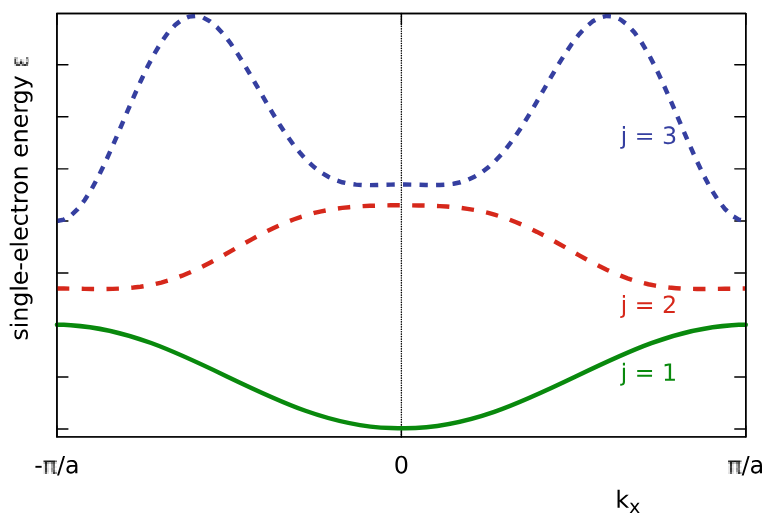
\includegraphics[width = 0.50 \textwidth]{en-band.png}
	\caption{First three energy bands for a 1D lattice.}
	\label{en-band}
\end{figure}

\subsection{Energy bands}

Facendo variare $ \ve{k} $ nella prima BZ, gli stati stazionari $ u_{j,\ve{k}}(\ve{r}) $ cambiano analiticamente con $ \ve{k} $, così da poter assumere una dipendenza liscia di $ u_{j,\ve{k}}(\ve{r}) $ da $ \ve{k} $. Di conseguenza, anche $ E_{j,\ve{k}} = E_j(\ve{k}) $ è una funzione liscia di $ \ve{k} $: per al variare di $ j \in \N $, si parla di \textit{energy bands}, in quanto fissato $ j \in \N $ gli autovalori $ E_j(\ve{k}) $ spannano un intervallo continuo di energie al variare di $ \ve{k} $ nella prima BZ. Come si vede in Fig. \ref{en-band}, i range spannati da due bands successive $ E_j(\ve{k} $ ed $ E_{j+1}(\ve{k}) $ possono sia sovrapporsi che rimanere separati: nel secondo caso, si parla di \textit{band gaps}. Si vede quindi che la principale conseguenza del teorema di Bloch è che lo spettro energetico degli elettroni in un solido cristallino è formato da energy bands continue separate da intervalli di energie proibite (band gaps): questo è un comportamento intermedio tra gli elettroni negli atomi (spettro discreto) e gli elettroni liberi (spettro continuo).

\subsubsection{Modello a onde piane}

Dato che all'interno del cristallo il potenziale nucleare $ V_{ne} $ è schermato dalla repulsione elettronica $ V_{ee} $, il potenziale effettivo $ V_\text{eff} $ è abbastanza piccolo (eccetto che vicino ai nuclei atomici) da poter approssimare gli autostati degli elettroni con quelli di particella libera. Questi sono gli autostati del momento lineare $ \ket{\ve{k}} : \hat{\ve{p}} \ket{\ve{k}} = \hbar \ve{k} \ket{\ve{k}} $ (opportunamente normalizzati come $ \braket{\ve{k} | \ve{k}'} = \delta_{\ve{k}, \ve{k}'} $), così da poter scrivere gli autostati elettronici come:
\begin{equation}
	\ket{\phi} = \sum_\ve{k} c_\ve{k} \ket{\ve{k}}
\end{equation}
L'equazione elettronica può quindi essere riscritta come (proiettando su $ \ket{\ve{k}} $):
\begin{equation}
	\sum_{\ve{k}'} \left[ \frac{\hbar^2 k^2}{2m_e} \delta_{\ve{k},\ve{k}'} + \braket{\ve{k} | V_\text{eff} | \ve{k}'} \right] c_{\ve{k}'} = E_\ve{k} \sum_{\ve{k}'} \delta_{\ve{k},\ve{k}'} c_{\ve{k}'}
\end{equation}
Per l'elemento di matrice del potenziale effettivo si trova:
\begin{equation}
	\braket{\ve{k} | V_\text{eff} | \ve{k}'} = \mathcal{N} \int \dd^3r\, e^{i (\ve{k}' - \ve{k}) \cdot \ve{r}} V_\text{eff}(\ve{r}) \eqdef \tilde{V}_\text{eff}(\ve{k} - \ve{k}')
\end{equation}
Essendo il potenziale periodico con stessa periodicità del reticolo cristallino, la sua trasformata di Fourier è in realtà una serie discreta sul reticolo reciproco: $ \tilde{V}_\text{eff}(\ve{k} - \ve{k}') $ si annulla a meno che $ \ve{k} - \ve{k}' = \ve{G} $. Ciò significa che la maggior parte degli elementi off-diagonal di $ V_\text{eff} $ si annullano: dato un $ \ve{k} $ nella prima BZ, il potenziale accoppia lo stato $ \ket{\ve{k}} $ solo a stati $ \ket{\ve{k}'} : \ve{k}' = \ve{k} - \ve{G} $, con $ \ve{G} $ nel reticolo reciproco. Trattando separatamente ciascun sottospazio a $ \ve{k} $ fissato (ovvero l'insieme $ \{\ket{\ve{k} + \ve{G}} : \ve{G} \in \text{reticolo reciproco}\} $), quindi, l'equazione elettronica può essere espressa come:
\begin{equation}
	\begin{bmatrix}
		\ddots & \vdots & \vdots & \vdots &  \\
		\dots & E_{\ve{k} + \ve{G}_1}^{(0)} + \tilde{V}_\text{eff}(\ve{0}) & \tilde{V}_\text{eff}(\ve{G}_1 - \ve{G}_2) & \tilde{V}_\text{eff}(\ve{G}_1 - \ve{G}_2) & \dots \\
		\dots & \tilde{V}_\text{eff}(\ve{G}_2 - \ve{G}_1) & E_{\ve{k} + \ve{G}_2}^{(0)} + \tilde{V}_\text{eff}(\ve{0}) & \tilde{V}_\text{eff}(\ve{G}_2 - \ve{G}_3) & \dots \\
		\dots & \tilde{V}_\text{eff}(\ve{G}_3 - \ve{G}_1) & \tilde{V}_\text{eff}(\ve{G}_3 - \ve{G}_2) & E_{\ve{k} + \ve{G}_3}^{(0)} + \tilde{V}_\text{eff}(\ve{0}) & \dots \\
		 & \vdots & \vdots & \vdots & \ddots
	\end{bmatrix}
	\begin{pmatrix}
		\vdots \\ c_{\ve{k} + \ve{G}_1} \\ c_{\ve{k} + \ve{G}_2} \\ c_{\ve{k} + \ve{G}_3} \\ \vdots
	\end{pmatrix}
	= E_\ve{k}
	\begin{pmatrix}
		\vdots \\ c_{\ve{k} + \ve{G}_1} \\ c_{\ve{k} + \ve{G}_2} \\ c_{\ve{k} + \ve{G}_3} \\ \vdots
	\end{pmatrix}
	\label{eq:mat-el-eq}
\end{equation}
dove l'energia all'ordine zero è quella dell'elettrone libero:
\begin{equation}
	E_\ve{k}^{(0)} = \frac{\hbar^2 k^2}{2m_e}
\end{equation}
L'Eq. \ref{eq:mat-el-eq} va diagonalizzata separatamente per ciascun $ \ve{k} $ nella prima BZ. La diagonalizzazione è banale nel caso di potenziale costante senza elementi off-diagonal $ \tilde{V}_\text{eff}(\ve{G} \neq \ve{0}) = 0 $: in tal caso, gli autostati energetici sono proprio le onde piane $ \ket{\ve{k} + \ve{G}_j} $, con autovalori energetici shiftati dal potenziale $ E_{j,\ve{k}} = E_{\ve{k} + \ve{G}_j}^{(0)} + \tilde{V}_\text{eff}(\ve{0}) $. \\
Nei cristalli reali, però, ci saranno molti termini off-diagonal non-nulli: in tal caso, gli autostati energetici sono combinazioni lineari delle onde piane $ \ket{\ve{k} + \ve{G}_j} $ e vengono trovati numericamente. \\
Un caso analiticamente affrontabile è quello di potenziale debole: precisamente, esso si verifica quando i termini off-diagonal sono piccoli rispetto alle separazioni diagonali, ovvero:
\begin{equation}
	\abs{\tilde{V}_\text{eff}(\ve{G}_1 - \ve{G}_2)} \ll \abs{E_{\ve{k} + \ve{G}_1}^{(0)} - E_{\ve{k} + \ve{G}_2}^{(0)}}
\end{equation}
In tale condizione, l'energia al prim'ordine è $ E_{j,\ve{G}}^{(1)} \approx E_{\ve{k} + \ve{G}_j}^{(0)} + \tilde{V}_\text{eff}(\ve{0}) $ e gli elementi off-diagonal determinano una piccola perturbazione al second'ordine:
\begin{equation}
	E_{j,\ve{k}}^{(2)} = E_{j,\ve{k}}^{(1)} + \sum_{\ell \neq j} \frac{\abs{\braket{\ve{k} + \ve{G}_j | V_\text{eff} | \ve{k} + \ve{G}_\ell}}^2}{E_{\ve{k} + \ve{G}_j}^{(0)} - E_{\ve{k} + \ve{G}_\ell}^{(0)}} = E_{j,\ve{k}}^{(1)} + \sum_{\ell \neq j} \frac{\abs{\tilde{V}_\text{eff}(\ve{G}_j - \ve{G}_\ell)}^2}{E_{\ve{k} + \ve{G}_j}^{(0)} - E_{\ve{k} + \ve{G}_\ell}^{(0)}}
\end{equation}
Questa correzione, però, non è applicabile nei punti in cui $ E_{\ve{k} + \ve{G}_j}^{(0)} \simeq E_{\ve{k} + \ve{G}_\ell}^{(0)} $ (evidenziati in Fig. \ref{band-par}): in questi punti, i termini off-diabonal diventano grandi e l'andamento risulta molto diverso da quello parabolico. Nei punti in cui due stati $ \ket{\ve{k} + \ve{G}_j} , \ket{\ve{k} + \ve{G}_\ell} $ diventano quasi degeneri, le band energies approssimate si possono calcolare diagonalizzando le (sotto)matrice:
\begin{equation*}
	\begin{bmatrix}
		E_{\ve{k} + \ve{G}_j}^{(0)} + \tilde{V}_\text{eff}(\ve{0}) & \tilde{V}_\text{eff}(\ve{G}_j - \ve{G}_\ell) \\
		\tilde{V}_\text{eff}(\ve{G}_\ell - \ve{G}_j) & E_{\ve{k} + \ve{G}_\ell}^{(0)} + \tilde{V}_\text{eff}(\ve{0})
	\end{bmatrix}
	\equiv
	\begin{bmatrix}
		E_{j,\ve{k}}^{(1)} & \Delta \\
		\Delta^* & E_{\ell,\ve{k}}^{(1)}
	\end{bmatrix}
\end{equation*}
Si trova che il coupling term $ \Delta $ induce una repulsione tra bande (formando gaps), le quali si trovano sempre a distanze energetiche pari o superiori a $ 2\abs{\Delta} = \abs{2\tilde{V}_\text{eff}(\ve{G}_j - \ve{G}_\ell} $, come riportato in Fig. \ref{band-gap}.

\begin{figure}
	\centering
	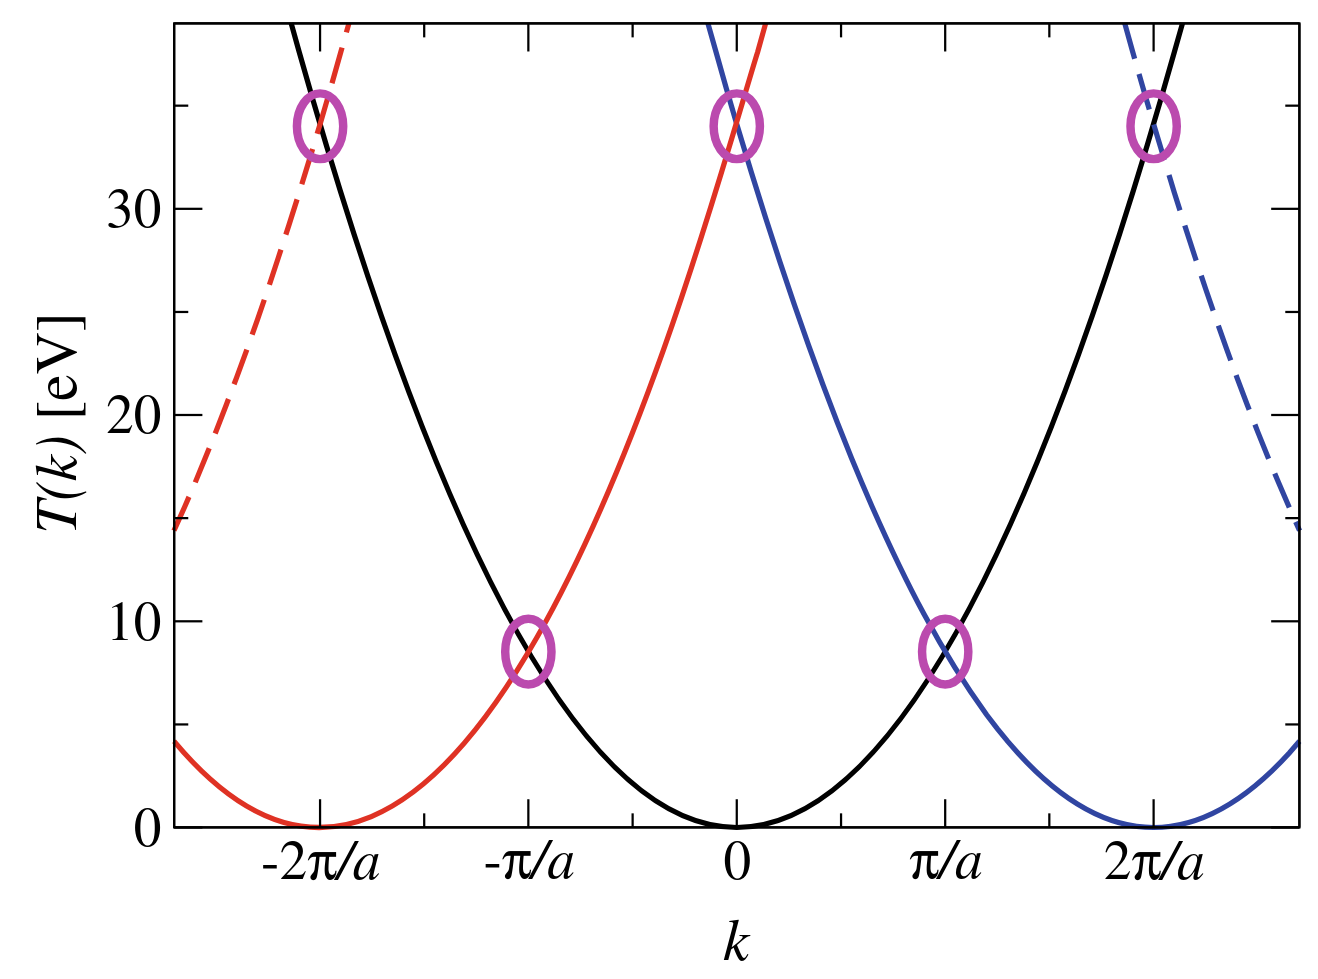
\includegraphics[width = 0.50 \textwidth]{band-par.png}
	\caption{1D free-electron parabolas $ E_{k + G_j}^{(0)} $, with $ G_j = \frac{2\pi}{a} j $: $ j = 0 $ in black, $ j = 1 $ in blue, $ j = 2 $ dashed in blue, $ j = -1 $ in red and $ j = -2 $ dashed in red.}
	\label{band-par}
\end{figure}
\begin{figure}
	\centering
	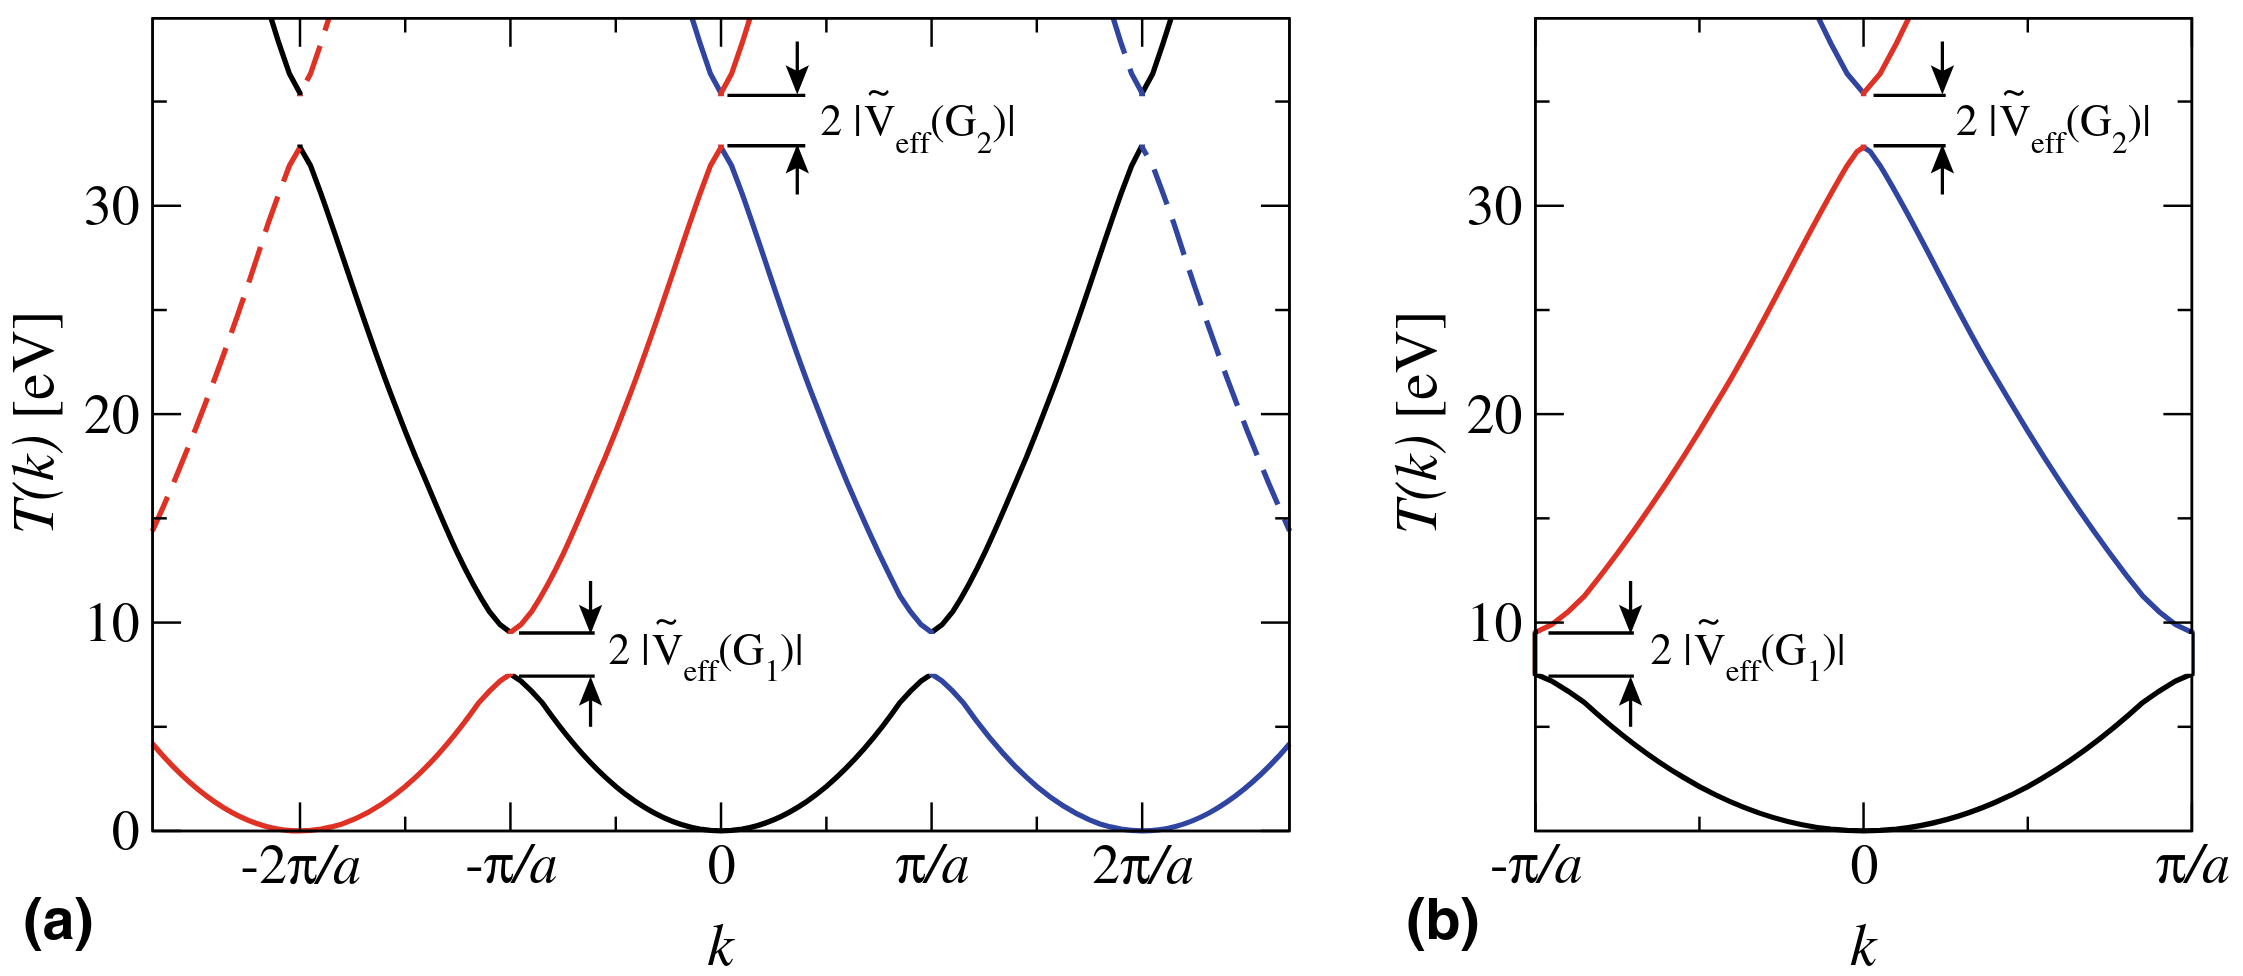
\includegraphics[width = 0.70 \textwidth]{band-gap.png}
	\caption{$ \abs{2\tilde{V}_\text{eff}(G_j)} $-wide gaps at each degeneracy point $ k = \frac{1}{2} G_j $, with the first BZ in detail.}
	\label{band-gap}
\end{figure}

Il modello a onde piane mostra chiaramente la formazione di band gaps, ovvero intervalli di energie proibite che separando le energy bands. In Fig. \ref{band-par}-\ref{band-gap} si vede come in 1D il potenziale periodico apre dei gap in tutti i punti $ k = \frac{1}{2} G $. In generale, in 3D, i gap si aprono in tutti i punti $ \ve{k} : \abs{\ve{k} + \ve{G}} = \abs{\ve{k}} $, per un qualche $ \ve{G} \in \text{reticolo reciproco} $: questa è proprio la condizione di Bragg per la diffrazione (Eq. \ref{eq:bragg-diffr}). Si noti che non sempre il potenziale periodico va a creare delle band gaps ben definite: può capitare, infatti, che un range di energie proibite per una certa direzione $ \ve{k} $ sia invece permessa per un'altra direzione $ \ve{k}' $. \\
Si vede che, nel modello a onde piane, l'indice $ j $ di una banda rappresenta semplicemente il numero di bande energeticamente sottostanti ad essa.

\subsubsection{Modello di Kronig-Penney}

\begin{figure}[!b]
	\centering
	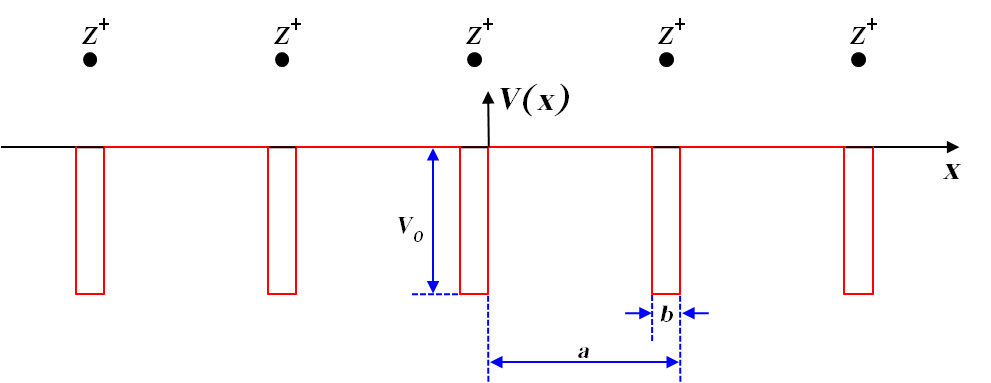
\includegraphics[width = 0.70 \textwidth]{kr-pen.png}
	\caption{Kronig-Penney model for the periodic potential.}
	\label{kr-pen}
\end{figure}

Una trattazione diversa è possibile grazie al modello di Kronig-Penney per il potenziale periodico. Grazie alle condizioni di periodicità, si può restringere la trattazione alla cella primaria, e nel caso 1D vale:
\begin{equation}
	V(x) =
	\begin{cases}
		-V_0 & -b < x < 0 \\
		0 & 0 < x < a-b
	\end{cases}
\end{equation}
La trattazione è analoga a quella della particella in una buca finita di potenziale, ma con diverse condizioni al contorno. In particolare, per un elettrone di energia $ E $, si trova:
\begin{equation}
	\psi(x) =
	\begin{cases}
		A e^{i \alpha x} + B e^{-i \alpha x} & -b < x < 0 \\
		C e^{i \beta x} + D e^{-i \beta x} & 0 < x < a-b
	\end{cases}
\end{equation}
con:
\begin{equation}
	\alpha^2 \equiv \frac{2m (E + V_0)}{\hbar^2}
	\qquad \qquad
	\beta^2 \equiv \frac{2m E}{\hbar^2}
\end{equation}
Si devono imporre condizioni di raccordo e periodicità, ovvero:
\begin{equation}
	\psi(0^-) = \psi(0^+)
	\qquad \qquad
	\psi'(0^-) = \psi'(0^+)
\end{equation}
\begin{equation}
	\psi(-b) = \psi(a-b)
	\qquad \qquad
	\psi'(-b) = \psi'(a-b)
\end{equation}
Dal teorema di Bloch $ \psi(x) = e^{ikx} u_k(x) $, dunque imponendo le condizioni periodiche si trova la condizione:
\begin{equation}
	\cos (ka) = \cos(\beta b) \cos (\alpha(a-b)) - \frac{\alpha^2 + \beta^2}{2\alpha \beta} \sin(\beta b) \sin(\alpha (a-b))
\end{equation}
Prendendo il limite di queste barriere di potenziale a $ \delta $ di Dirac, ovvero $ b \rightarrow 0 , V_0 \rightarrow \infty : bV_0 = \text{const.} $, si trova:
\begin{equation}
	\cos(ka) = \cos(\alpha a) + p \sinc(\alpha a)
	\qquad \qquad
	p \equiv \frac{m V_0 ba}{\hbar^2}
\end{equation}
Questa equazione ha soluzione solo se $ \abs{\cos(\alpha a) + p \sinc(\alpha a)} \le 1 $: essendo $ \alpha a \propto \sqrt{E} $, ciò significa che ci sono dei valori energetici per cui non c'è soluzione, ovvero si formano delle band gaps (Fig. \ref{kr-pen-en}).

\begin{figure}
	\centering
	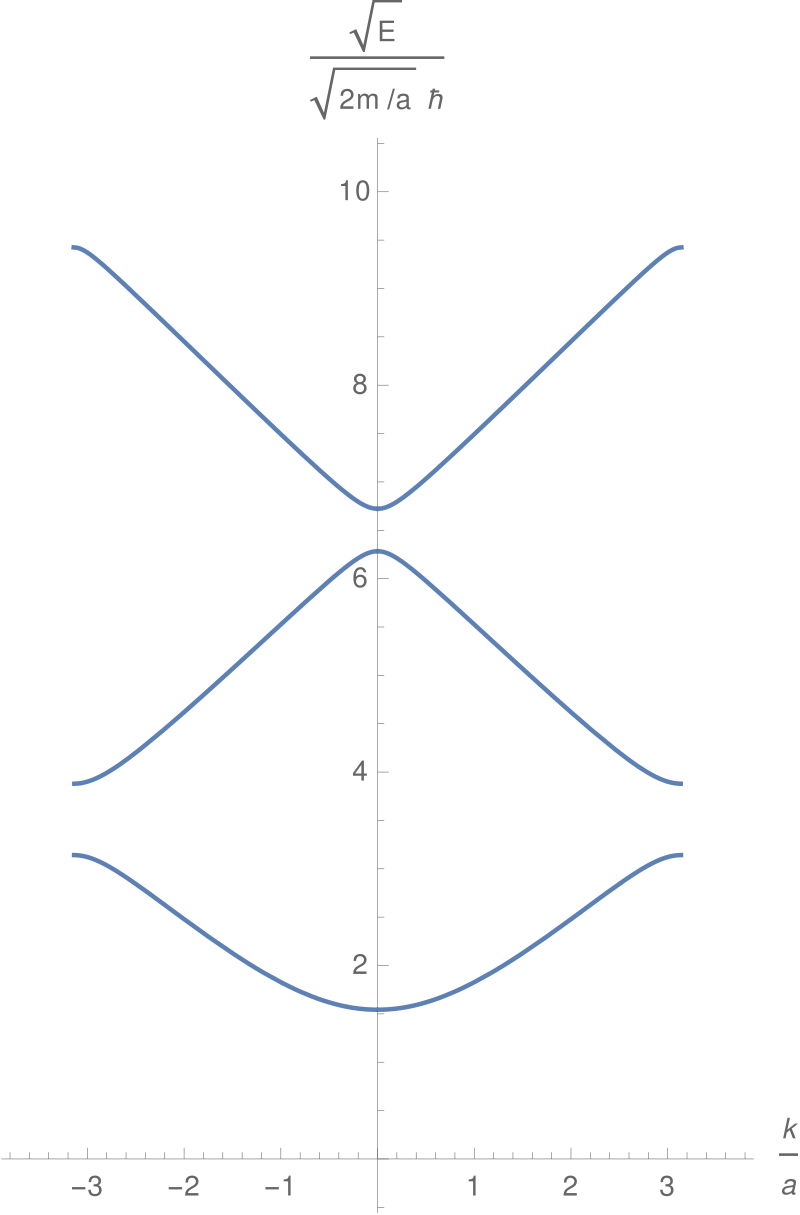
\includegraphics[width = 0.30 \textwidth]{kr-pen-en.png}
	\caption{Energy bands for the Kronig-Penney model.}
	\label{kr-pen-en}
\end{figure}

\subsubsection{Tight-binding model}

Si consideri un reticolo cristallino 1D con atomi posizionati in punti equispaziati $ t_n \equiv na $: vicino ciascuno di essi, il potenziale effettivo sarà approssimato da quello di un singolo nucleo isolato, dunque è possibile ottenere la funzione d'onda elettronica a partire da quelle atomiche. In questo modo, le funzioni d'onda di Bloch sono delle generalizzazioni degli orbitali leganti/anti-leganti ottenuti tramite LCAO (si pensa al solido come ad una grossa molecola): questo sistema è appropriato per elementi che contengono solo orbitali $ \text{s} $, mentre risulta poco adatto a descrivere stati metallici estesi. \\
Si considerino le funzioni d'onda atomiche per ciascun atomo $ \phi_\text{a}(x-t_n) $. Essendo il sistema invariante per traslazioni, gli elementi diabonali di matrice dell'Hamiltoniana sono tutti uguali:
\begin{equation}
	\braket{\phi_\text{a}(x-t_n) | \mathcal{H} | \phi_\text{a}(x-t_n)} = E_0
\end{equation}
Si definisce inoltre l'\textit{integrale di Hopping}:
\begin{equation}
	\gamma \defeq \braket{\phi_\text{a}(x-t_n) | \mathcal{H} | \phi_\text{a}(x-t_{n+1})}
\end{equation}
Essendo i potenziali atomici attrattivi, si ha $ \gamma < 0 $. Per costruire una funzione d'onda periodica estesa a partire da questi orbitali atomici localizzati, si può utilizzare il teorema di Bloch, trovando la \textit{somma di Bloch}:
\begin{equation}
	\phi_k(x) = \frac{1}{\sqrt{N}} \sum_{n = 1}^N e^{i k t_n} \phi_\text{a}(x-t_n)
\end{equation}
Si vede infatti che $ \phi_k(x+a) = e^{ika} \phi_k(x) $, rispettando il teorema di Bloch. Lo spettro energetico sarà:
\begin{equation}
	E(k) = \braket{\phi_k | \mathcal{H} | \phi_k} = E_0 + 2 \gamma \cos(ka)
\end{equation}
Attorno al minimo si recupera la forma parabolica:
\begin{equation}
	E(k) \simeq E_0 + 2\gamma - \gamma a^2 k^2 \equiv E_0 + 2\gamma + \frac{\hbar^2 k^2}{2\mu}
	\qquad \qquad
	\mu \equiv \frac{\hbar^2}{2 \abs{\gamma} a^2}
\end{equation}
dove si è definita la massa efficace $ \mu $. Si vede che $ \mu $ è piccola per $ \abs{\gamma} $ grande: le masse piccole sono più soggette ai campi esterni (in quanto accellerano più facilmente).

\subsection{Riempimento delle bande}

\begin{figure}
	\centering
	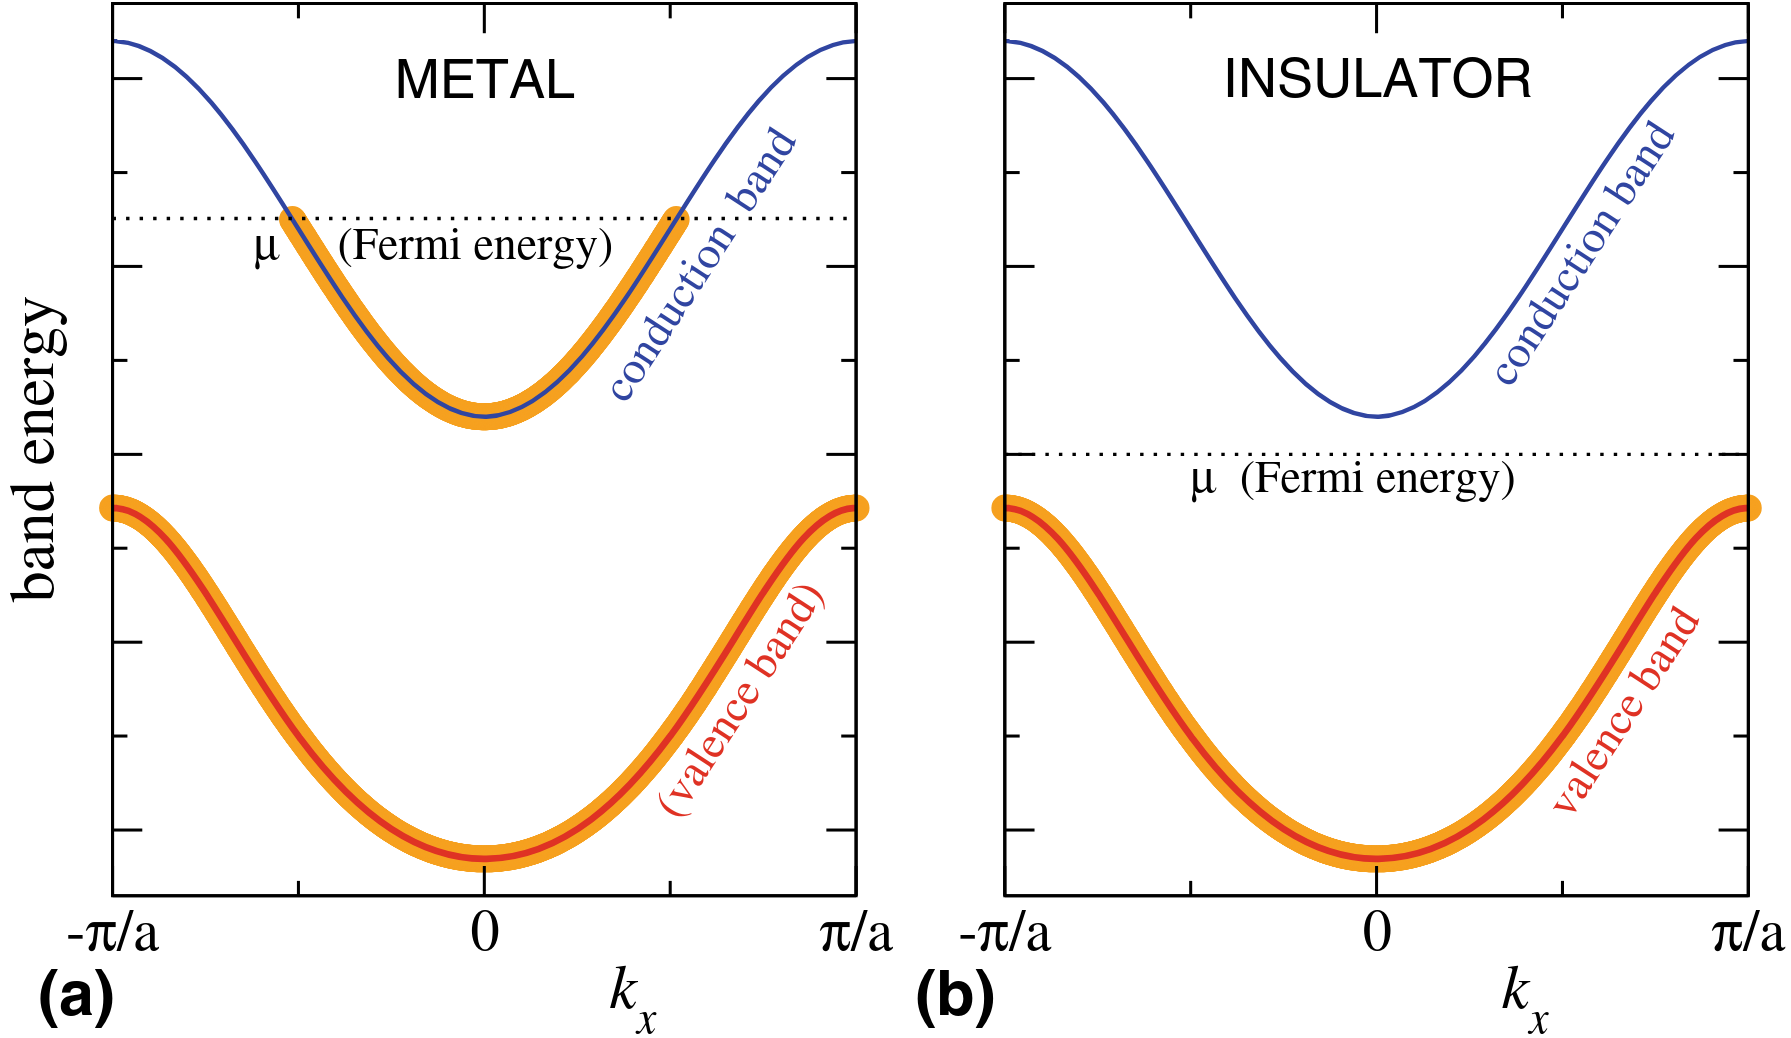
\includegraphics[width = 0.50 \textwidth]{met-ins.png}
	\caption{The two fundamental $ T = 0 $ band-fillinf schemes: metal and insulator.}
	\label{met-ins}
\end{figure}

Il ground state ($ T = 0 $) di un sistema di elettroni indipendenti in un potenziale periodico si ottiene riempiendo gli stati single-particle nelle energy bands fino all'energia di Fermi $ \mu $, come nel modello a fermioni liberi. \\
In base al numero di elettroni nel solido, l'energia di Fermi può intersecare una o più energy bands o capitare in mezzo ad una band gap (vedere Fig. \ref{met-ins}): nel primo caso, gli elettroni nelle band occupate parzialmente possono acquisire energia d'eccitazione da campi esterni, così accellerando e conducendo corrente elettrica (\textit{metallo}); nel secondo caso, invece, gli elettroni in una band completa rimangono congelati per il principio d'esclusione, e le eccitazioni richiedono energie dell'ordine della band gap (\textit{isolante}). In generale, l'energy band completamente riempita più alta viene detta \textit{banda di valenza}, mentre quella parzialmente riempita più bassa \textit{banda di conduzione}. \\
Per capire come si distribuiscono gli elettroni nelle energy bands, si consideri una porzione di cristallo di volume $ V = N_1 N_2 N_3 V_c $, la quale si estende per $ N_1 / N_2 / N_3 $ periodi nella direzione $ \ve{a}_1 / \ve{a}_2 / \ve{a}_3 $. Applicando la condizione di periodicità $ \psi-{j,\ve{k}}(\ve{r}) = \psi_{j,\ve{k}}(\ve{r} + N_i \ve{a}_i) $ si trova:
\begin{equation*}
	\ve{k} = \frac{n_1}{N_1} \ve{b}_1 + \frac{n_2}{N_2} \ve{b}_2 + \frac{n_3}{N_3} \ve{b}_3
	\qquad \qquad
	n_i = - \frac{N_i}{2} + 1 , - \frac{N_i}{2} + 2 , \dots , \frac{N_i}{2} -1 , \frac{N_i}{2}
\end{equation*}
I valori possibili di $ \ve{k} $ sono quindi $ N = N_1 N_2 N_3 $: questi diventano densi e riempiono la prima BZ nel limite $ N_i \rightarrow \infty $ (cristallo ideale infinito). Ciascuno stato nella banda $ j $ può ospitare due elettroni (degenerazione da spin), dunque in totale la banda ha $ 2N $ stati single-particle.

\begin{proposition}{Occupazione delle bande}{}
	Detto $ m $ il numero di elettroni in ciascun atomo ed $ n_c $ il numero di atomi per cella, il numero di bande occupate è $ \frac{1}{2} m n_c $.

	\tcblower

	\begin{proof}
		Essendo presenti $ N $ celle nel volume $ V $, il numero totale di atomi in $ V $ è $ m n_c N $: ciascuna banda può ospitare $ 2N $ elettroni, dunque il numero di bande occupate è $ \frac{m n_c N}{2N} = \frac{1}{2} m n_c $.
	\end{proof}
\end{proposition}

Si hanno dunque due possibili casi, a seconda che il numero di elettroni per cella $ m n_c $ sia pari o dispari (vedere Fig. \ref{ne-na}):
\begin{itemize}
	\item $ m n_c $ pari: viene occupato un numero intero di bande, ovvero la banda di conduzione è vuota;
	\item $ m n_c $ dispari: l'ultima banda è semi-piena, ovvero ci sono degli elettroni nella banda di conduzione.
\end{itemize}

\begin{figure}
	\centering
	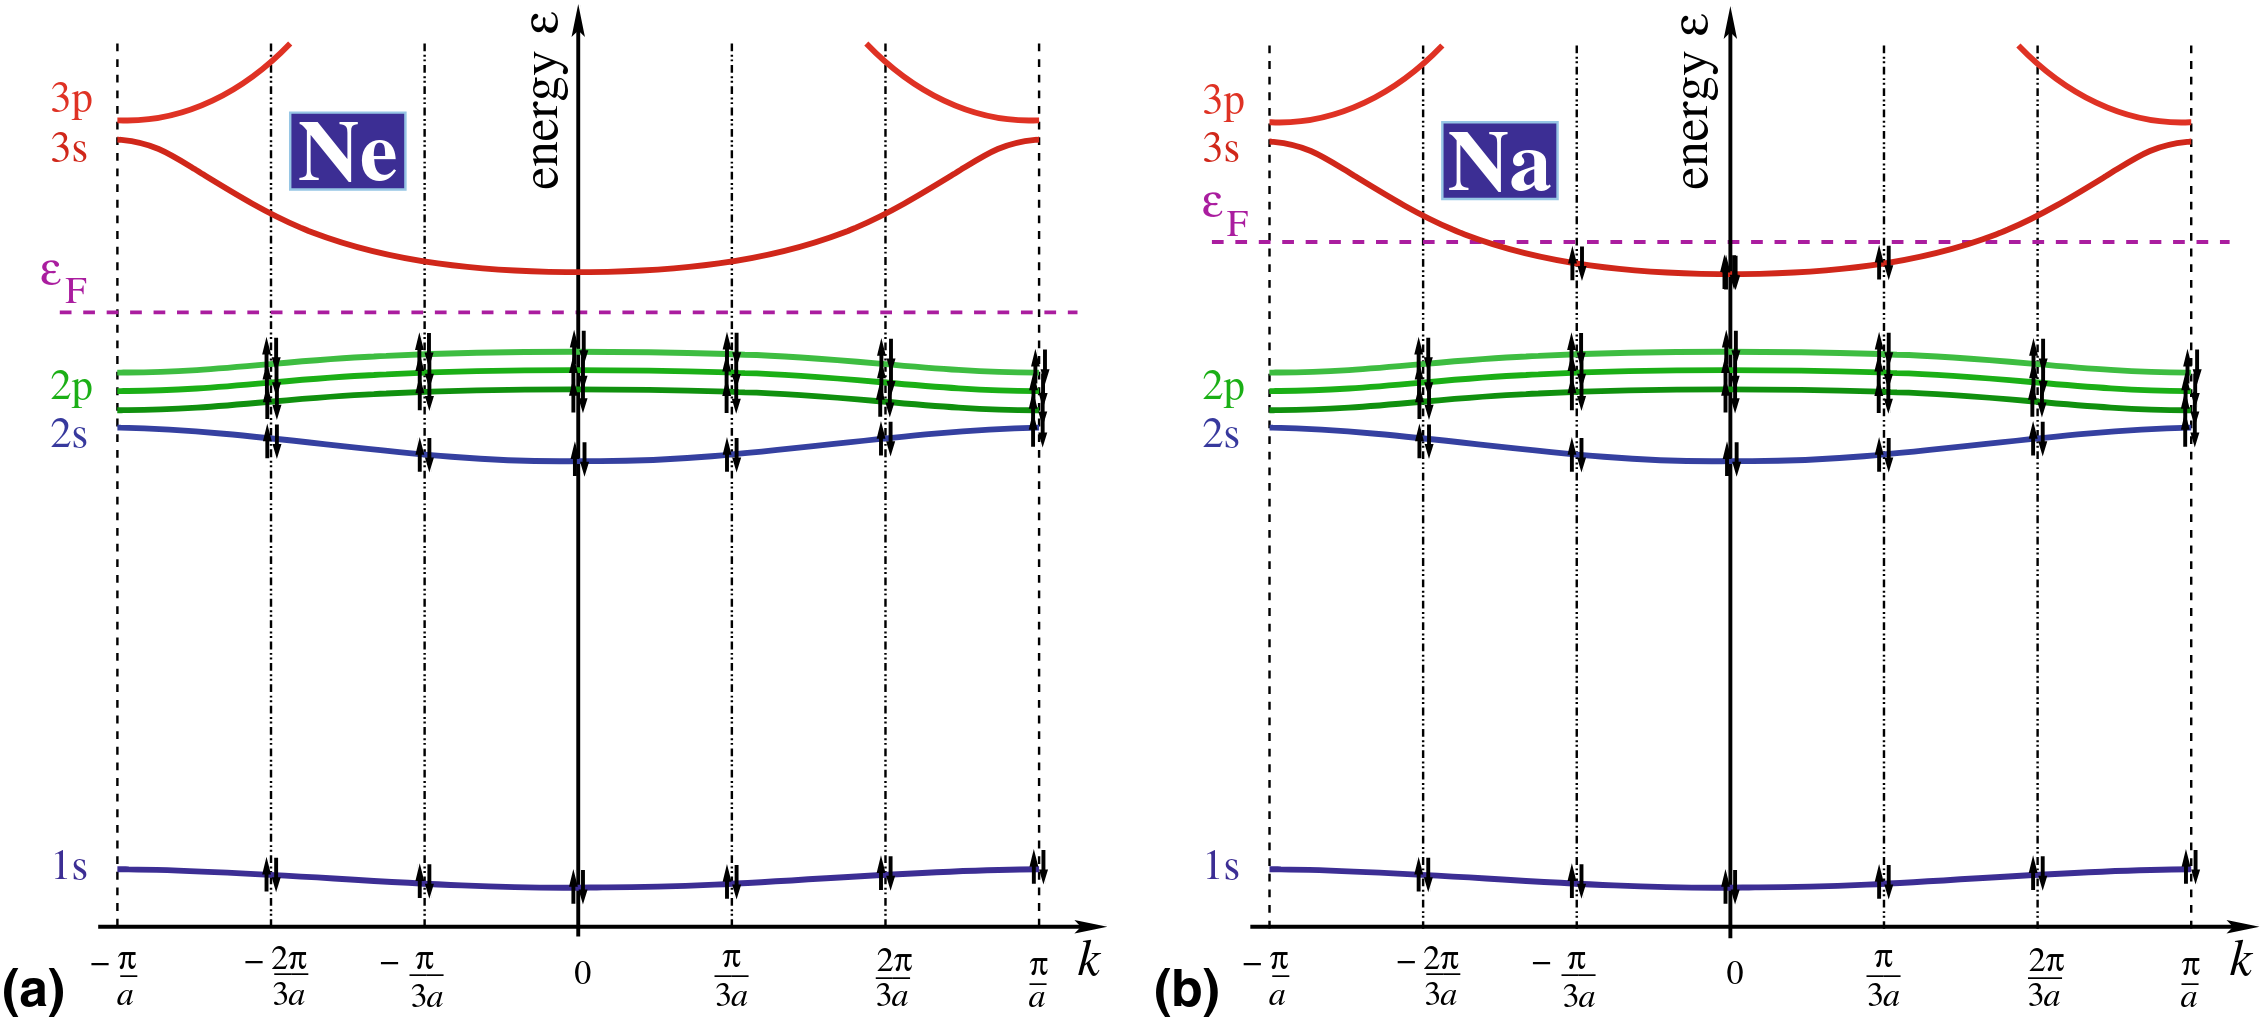
\includegraphics[width = 0.70 \textwidth]{ne-na.png}
	\caption{Filling of bands for 1D crystals of $ N = 6 $ atoms of $ \ch{Ne} $ and $ \ch{Na} $.}
	\label{ne-na}
\end{figure}

Si vede dunque che i cristalli con un numero dispari di elettroni per cella sono dei metalli, mentre quelli che ne hanno un numero pari possono essere sia isolanti che metalli: quest'ultimo caso si verifica quando la banda di valenza e quella di conduzione non sono separate da gap, dunque parte della banda di valenza è al di sopra dell'energia di Fermi e parte della banda di conduzione al di sotto di essa (si verifica nel gruppo 2 (metalli alcalino-terrosi) e nel gruppo 12 ($ \ch{Zn} $, $ \ch{Cd} $ e $ \ch{Hg} $)).

\subsubsection{Metalli}

I metalli presentano una particolare capacità di condurre corrente elettrica\footnotemark: in particolare, mostrano una conducibilità elettrica che decresce con $ T $.
A $ T = 0 $, la \textit{superficie di Fermi} $ E = \mu $ separa gli stati pieni da quelli vuoti nello spazio reciproco (dei $ \ve{k} $), generalizzando la sfera di Fermi per il gas ideale di fermioni.

\footnotetext{In realtà tutti i solidi possono condurre corrente elettrica: ciò che caratterizza i metalli è l'andamento decrescente della conducibilità elettrica all'aumentare della temperatura, a differenza della (piccola) conducibilità elettrica degli isolanti che invece aumenta con $ T $.}

Adottando un approccio semiclassico, si può studiare il moto degli elettroni rappresentandoli come pacchetti d'onda, ovvero sovrapposizioni di stati di Bloch relativi ad una stessa banda $ j $. Il moto di un pacchetto d'onda soggetto ad un campo elettromagnetico esterno è governato da:
\begin{equation}
	\dot{\ve{r}} \equiv \ve{v}_j(\ve{k}) = \frac{1}{\hbar} \nabla_\ve{k} E_{j,\ve{k}}
	\label{eq:met-1}
\end{equation}
\begin{equation}
	\hbar \dot{\ve{k}} = -q_e \left[ \ve{E}_\text{ext}(t,\ve{r}) + \ve{v}_j(\ve {k}) \times \ve{B}_\text{ext}(t,\ve{r}) \right]
	\label{eq:met-2}
\end{equation}
dove si assume che il campo esterno vari lentamente nel tempo sulla scala della grandezza del pacchetto (tipicamente molto maggiore della dimensione della cella primaria del reticolo, in quanto si suppone il pacchetto centrato in un valore di del numero d'onda ben definito). \\
La velocità $ \ve{v}_j $ è la velocità del centro di massa dell'elettrone, ovvero la velocità di gruppo del wave-packet: l'Eq. \ref{eq:met-1} esprime il fatto che un pacchetto d'onda con relazione di dispersione $ \omega = \omega(\ve{k}) $ ha una velocità di gruppo $ \ve{v}_g = \nabla_\ve{k} \omega(\ve{k}) $, dato che per l'elettrone $ \omega(\ve{k}) = \frac{1}{\hbar} E_{j,\ve{k}} $ (si noti che per l'elettrone libero $ E_{j,\ve{k}} = \hbar^2 k^2 / (2m_e) $, quindi si trova giustamente $ \ve{v}_j(\ve{k}) = \hbar \ve{k} / m_e $). \\
L'Eq. \ref{eq:met-2} ricorda l'equazione classica per una particella carica in un campo elettromagnetico esterno (forza di Lorentz): il potenziale periodico del cristallo induce una dipendenza non-banale $ \ve{v}_j = \ve{v}_j(\ve{k}) $, dunque il \textit{momento cristallino} $ \hbar \ve{k} $ non rappresenta il momento reale dell'elettrone\footnotemark. Ciò nonostante, $ \ve{k} $ è comunque una costante del moto, dunque continua ad essere un buon numero quantico.

\footnotetext{Il momento cristallino non è autovalore dell'operatore $ -i \hbar \nabla_\ve{r} $, dato che:
\begin{equation*}
	-i \hbar \nabla_\ve{r} \left[ e^{i \ve{k} \cdot \ve{r}} u_\ve{k}(\ve{r}) \right] = \hbar \ve{k} e^{i \ve{k} \cdot \ve{r}} u_\ve{k}(\ve{r}) -i \hbar e^{i \ve{k} \cdot \ve{r}} \nabla_\ve{r} u_\ve{k}(\ve{r}) \neq \hbar \ve{k} e^{i \ve{k} \cdot \ve{r}} u_\ve{k}(\ve{r})
\end{equation*}
Prendendo il valore d'aspettazione, si vede che il momento dell'elettrone è il momento cristallino diminuito di una quantità che può essere vista come un momento medio efficace: quest'ultimo viene interpretato come un momento medio trasferito dall'elettrone al cristallo.
}

È possibile calcolare l'accellerazione di un elettrone, a partire dall'Eq. \ref{eq:met-1}:
\begin{equation*}
	\frac{\dd^2 \ve{r}}{\dd t^2} = \frac{\dd \ve{k}}{\dd t} \cdot \nabla_\ve{k} \ve{v}_j(\ve{k}) = \frac{1}{\hbar^2} \sum_{\alpha,\beta = 1}^3 \hat{\ve{e}}_\alpha \frac{\pa^2 E_{j,\ve{k}}}{\pa k_\alpha \pa k_\beta} \frac{\dd (\hbar k_\beta)}{\dd t} \equiv \sum_{\alpha,\beta = 1}^3 \hat{\ve{e}}_\alpha [m_\text{eff}^{-1}]_{\alpha,\beta} F_\beta
\end{equation*}
dove sono state definite la forza totale esterna agente sull'elettrone $ \ve{F} = \hbar \dot{\ve{k}} $ (Eq. \ref{eq:met-2}) e la \textit{massa efficace} $ m_\text{eff} $, definita tensorialmente tramite il suo inverso:
\begin{equation}
	[m_\text{eff}^{-1}]_{\alpha,\beta} = \frac{1}{\hbar^2} \frac{\pa^2 E_{j,\ve{k}}}{\pa k_\alpha \pa k_\beta}
\end{equation}
Questa massa può anche essere negativa o divergere, e per l'elettrone libero si trova correttamente $ m_\text{eff} = m_e $. In particolare, sulla superficie di Fermi (dove avviene il moto), gli elettroni si comportano come se avessero massa $ m_\text{eff} $ (opportuna media sulle componenti del tensore), la quale è proporzionale alla curvatura dell'energy band.

\paragraph{Corrente elettrica}

Con l'approccio semiclassico, è facile vedere che un'energy band completamente piena non conduce corrente. Essendo la densità di corrente trasportata da un wave-packet $ \ve{j}_p(\ve{k}) = -q_e \ve{v}_j(\ve{k}) / V $ e ricordando l'Eq. \ref{eq:dens-k}, si trova:
\begin{equation*}
	\ve{J} = \int_\text{BZ} \dd^3k\, \ve{j}_p(\ve{k}) g_s g(\ve{k}) = - \frac{q_e}{4\pi^3 \hbar} \int_\text{BZ} \dd^3k\, \nabla_\ve{k} E_{j,\ve{k}} = \ve{0}
\end{equation*}
che si annulla poiché è l'integrale sul periodo del gradiente di una funzione periodica. Ciò spiega perché non si osserva un aumento della conducibilità elettrica negli elementi cristallini all'aumentare di $ Z $: ad esempio, $ \ch{Cu} $, $ \ch{Ag} $ ed $ \ch{Au} $ hanno conducibilità simili, nonostante il numero totale di elettroni molto diverso. \\
Concentrandosi sulle bande semi-piene, si noti che gli stati di Bloch sono stati stazionari in un cristallo perfetto: di conseguenza, se un wave-packet ha velocità di gruppo finita ($ \nabla_\ve{k} E_{l,\ve{k}} \neq \ve{0} $), allora essa rimarrà immutata mentre l'elettrone si sposta nel cristallo. Ciò significa che, nell'approccio semiclassico, le correnti si dovrebbero propagare nel metallo come fossero nel vuoto, anche in assenza di un campo elettrico esterno: queste persistent current non vengono però osservate negli esperimenti.
Inoltre, secondo l'Eq. \ref{eq:met-2}, sotto l'effetto di un campo elettrico costante uniforme l'elettrone ha un moto ciclico nella prima BZ (ricordando le condizioni periodiche, si veda Fig. \ref{k-cycle}): queste sono note come \textit{oscillazioni di Bloch}. Di conseguenza, per l'Eq. \ref{eq:met-1}, la velocità è oscillante e genera correnti positive e negative per lo stesso periodo di tempo: ciò significa, che applicando un campo elettrico DC ad un filo metallico, si dovrebbe osservare una corrente AC. Questa è un'altra discrepanza con quanto viene osservato, in quanto la risposta dei metalli ad un campo elettrico esterno è dettata dalla legge di Ohm: $ \ve{J} = \sigma \ve{E} $, con $ \sigma $ conducibilità elettrica. \\
Queste discrepanza tra teoria semiclassica e realtà sono dovute al fatto che gli elettroni di Bloch, rappresentati da pacchetti d'onda, posti in un cristallo ideale possono muoversi all'infinito, senza dispersione d'energia. I cristalli reali, però, deviano da quelli ideali per la presenza di difetti e per il fatto che gli atomi non sono fissi nelle posizioni reticolari, ma possono oscillare attorno ad esse: ciò determina che gli elettroni di conduzione siano soggetti a fenomeni di scattering, in particolare a causa dell'interazione elettrone-fonone.

\begin{figure}
	\centering
	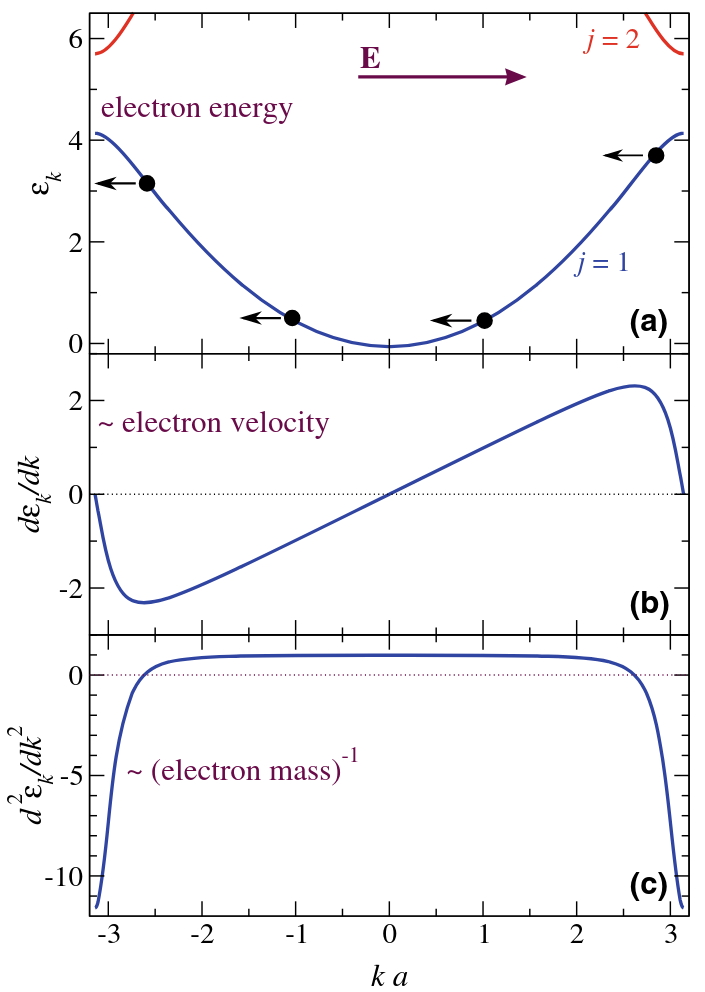
\includegraphics[width = 0.40 \textwidth]{k-cycle.png}
	\caption{Motion of an electron in the reciprocal lattice of a 1D crystal, under the action of a constant uniform electric field.}
	\label{k-cycle}
\end{figure}

Per metalli cristallini, il tempo medio $ \tau $ tra due collissioni di un elettrone (\textit{tempo libero medio} o tempo di rilassamento) è dell'ordine $ \tau \sim 10^{-13} \,\text{s} $, troppo breve perché l'elettrone raggiunga il bordo della prima BZ e mostri oscillazioni di Bloch\footnotemark.

\footnotetext{Per osservare le oscillazioni di Bloch servirebbe un cristallo estremamente puro a temperatura molto bassa, condizioni difficilmente ottenibili. In alternativa, si possono considerare i \textit{super-reticoli}, ovvero reticoli sovrapposti di materiali diversi, le cui celle si vanno ad alternare: ciò permette di rendere la cella primitiva più grande, ovvero di rimpicciolire la prima BZ. Si noti che sono necessari materiali tali per cui all'interfaccia non ci sia una grossa differenza di passi reticolari, così da non introdurre difetti.}

Mentre il campo elettrico esterno spinge gli elettroni ad occupare stati nella direzione di $ -q_e \ve{E}_\text{ext} $, le collisioni con difetti del cristallo e fononi tendono a riportare gli elettroni verso gli stati occupati all'equilibrio termico: dopo un transiente, l'effetto di $ \ve{E}_\text{eff} $ viene ridotto ad un piccolo shift $ \delta \ve{k} $ costante della superficie di Fermi rispetto alla sua configurazione all'equilibrio. Definendo $ \delta^3k $ il volume tra la superficie di Fermi all'equilibrio e quella shiftata, si può stimare la densità di corrente indotta da $ \ve{E}_\text{eff} $ come:
\begin{equation*}
	\ve{J} = - \frac{q_e}{4\pi^3} \int_{\delta^3k} \dd^3k\, \ve{v}_j(\ve{k}) \simeq - q_e \int_{\delta^3k} \dd^3k\, \hat{\ve{E}}_\text{ext} v_\text{F} \simeq -q_e v_\text{F} \hat{\ve{E}}_\text{eff} \delta^3k
\end{equation*}
dove si è approssimato l'integrale con la velocità di Fermi nella direzione del campo poiché sono coinvolti solo gli \textit{elettroni attivi}, ovvero quelli sulla superficie di Fermi. Osservando che nel tempo libero medio $ \tau $ l'elettrone varia il suo numero d'onda come $ \delta\ve{k} = -q_e \tau \ve{E}_\text{ext} / \hbar $ (Eq. \ref{eq:met-2}), si può stimare:
\begin{equation*}
	\delta^3k \simeq - \abs{\delta\ve{k}} k_\text{F}^2 \simeq - q_e \frac{\tau}{\hbar} \abs{\ve{E}_\text{ext}} k_\text{F}^2
\end{equation*}
dove il segno negativo indica che lo shift è opposto ad $ \ve{E}_\text{ext} $. Essendo $ v_\text{F} \simeq \hbar k_\text{F} / m_\text{eff} $ e ricordando l'Eq. \ref{eq:k-f}, si trova:
\begin{equation*}
	\ve{J} \simeq \frac{q_e^2 \tau}{m_e} \hat{\ve{E}}_\text{ext} \abs{\ve{E}_\text{ext}} k_\text{F}^3 \simeq \frac{q_e^2 \tau}{m_e} \frac{N}{V} \ve{E}
\end{equation*}
Ciò non è altro che la legge di Ohm con conducibilità elettrica pari a:
\begin{equation}
	\sigma = \frac{q_e^2 \tau}{m_e} \frac{N}{V}
\end{equation}
Grandezze tipiche sono $ \tau \sim 10^{-13} \,\text{s} $, $ v_\text{F} \sim 10^6 \,\text{m}/\text{s} $ e $ N/V \sim 10^{29} \,\text{m}^{-3} $: si stima dunque il cammino libero medio $ l \simeq \tau v_\text{F} \sim 100 \,\text{nm} $. All'aumentare della temperatura si osserva un aumento della resistivistà $ \rho = \sigma^{-1} $, ovvero una diminuzione del tempo libero medio $ \tau $: le collisioni diventano più frequenti quando il moto termico determina grandi spostamenti dei nuclei dalla loro posizione d'equilibrio\footnote{Il tempo libero medio è inversamente proporzionale al numero di fononi: $ \tau^{-1} \propto \sum_\varepsilon [n_\varepsilon]_\text{B} $. Ad energie termiche $ k_\text{B} T $ molto al di sopra dell'energia caratteristica dei fononi ($ \varepsilon \lesssim 100 \,\text{meV} $), il numero totale di fononi è lineare in $ T $: dall'Eq. \ref{eq:fer-dir-bos-ein} $ [n_\varepsilon]_\text{B} = (e^{\beta \varepsilon} - 1)^{-1} \simeq (\beta \varepsilon)^{-1} = k_\text{B} T / \varepsilon $. Di conseguenza, ad alte tempreature la resistività è lineare in $ T $, fatto osservato sperimentalmente.}.

\begin{figure}
	\centering
	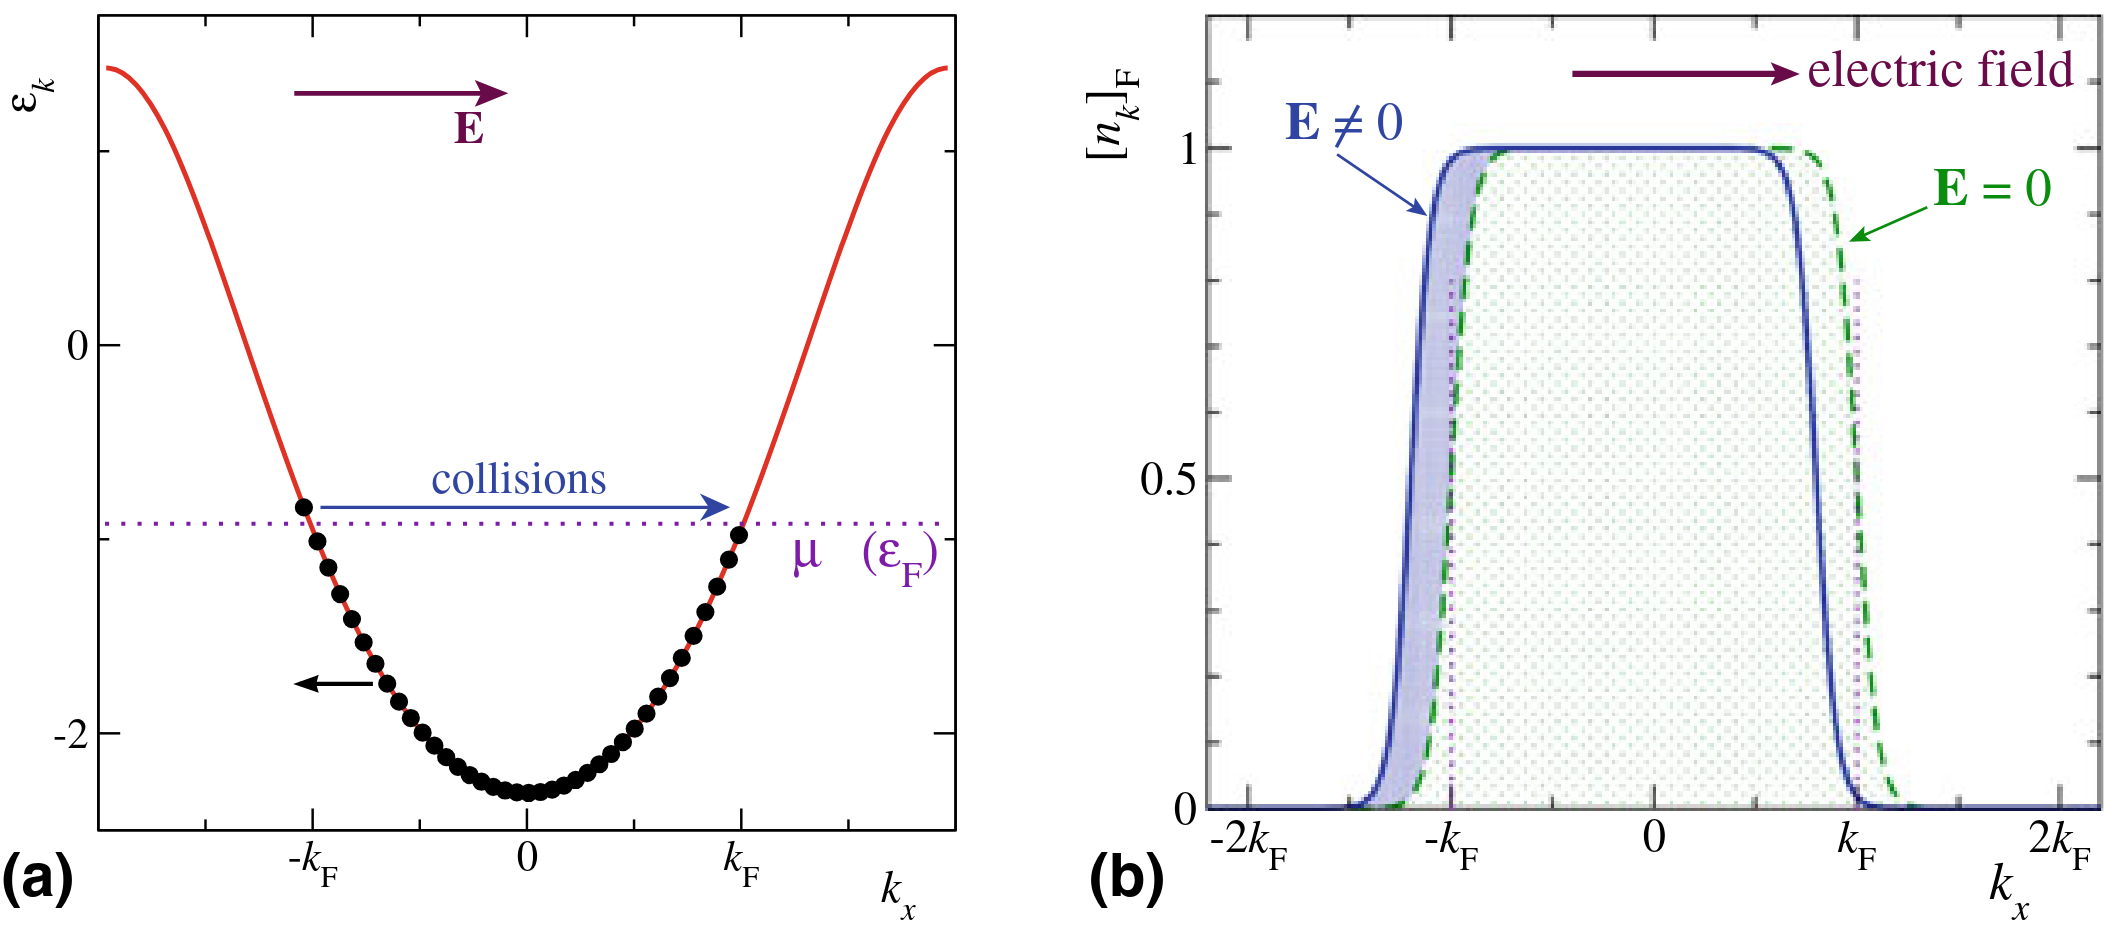
\includegraphics[width = 0.70 \textwidth]{therm-eq.png}
	\caption{Band occupation under the competing action oa a static electric field and collition with crystal defects and phonons.}
	\label{therm-eq}
\end{figure}
\begin{figure}
	\centering
	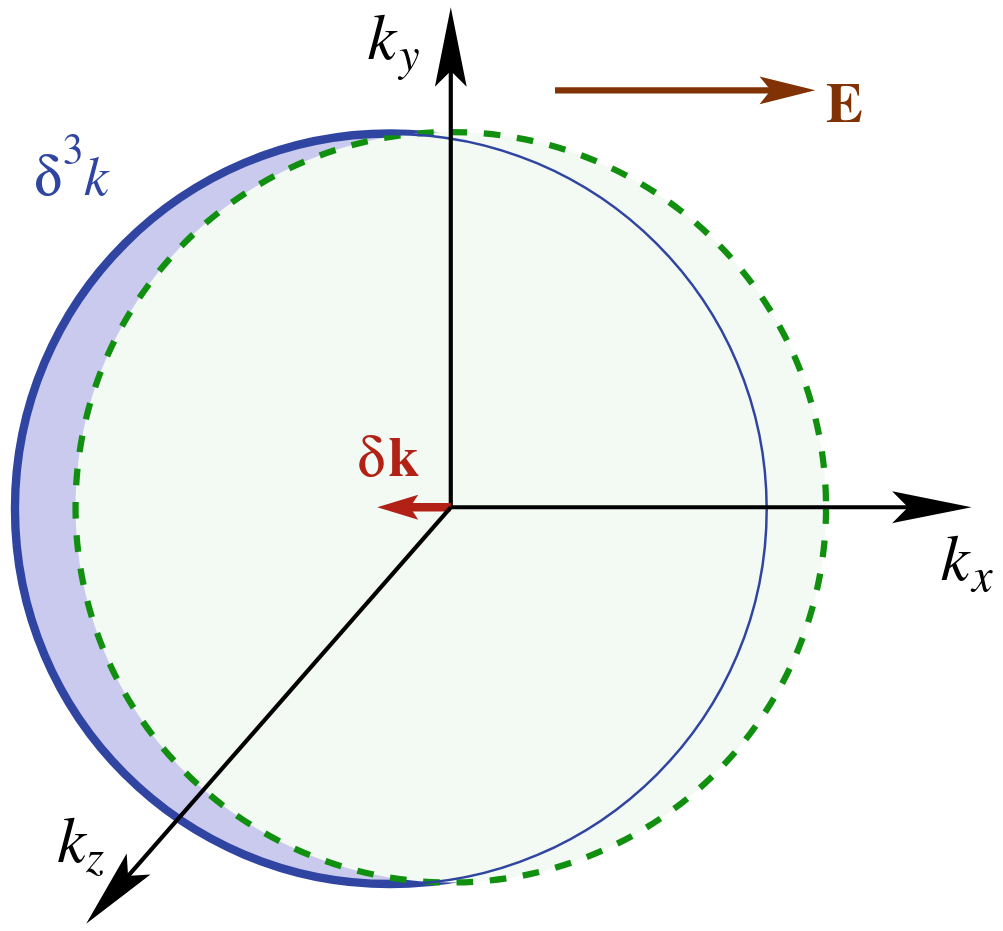
\includegraphics[width = 0.30 \textwidth]{fermi-sphere.png}
	\caption{Shift of the Fermi surface induced by a static electric field.}
	\label{f-sph}
\end{figure}

\subsubsection{Semiconduttori}

Negli isolanti, a differenza dei metalli, la densità dei portatori di carica (e dunque la conduttività elettrica) è proporzionale alla temperatura: oltre una certa temperatura, però, il moto dei portatori viene fortemente perturbato dall'agitazione termica, dunque $ \sigma $ torna a diminuire con l'aumentare di $ T $. Gli isolanti che a temperatura ambiente presentano una piccola conducibilità elettrica a temperatura ambiente (invece di $ \sigma = 0 $) vengono chiamati \textit{semiconduttori}: questi sono tipicamente cristalli in cui la gap tra la banda di valenza e quella di conduzione è larga $ \sim 1\ev $ a temperatura ambiente (es.: $ \ch{Si} $, $ \ch{Ge} $, etc.). \\
I semiconduttori presentano delle strutture cristalline diverse tra loro e, in virtù di queste differenze chimico-strutturali, le energy bands elettroniche di semiconduttori diversi presentano differenze qualitative e quantitative. In particolare, detti $ E_c $ il minimo della banda di conduzione ed $ E_v $ il massimo della banda di valenza, la gap $ \Delta = E_c - E_v $ può essere diretta, se $ E_c $ ed $ E_v $ sono nello stesso punto $ \ve{k} $, o indiretta, se si trovano in punti differenti. Dato che i fotoni, essendo massless, trasportano un momento piccolo, le transizioni ottiche coinvolgono sempre gap dirette: le transizioni indirette sono invece mediate da fononi, i quali però determinano interazioni al second'ordine poco probabili. I materiali a \textit{gap diretta} sono quelli in cui la gap più piccola è quella diretta, mentre i materiali a \textit{gap indiretta} hanno come gap minima quella indiretta: un esempio di quest'ultimi è il silicio, che ha una gap diretta $ \sim 3\ev $ ed una indiretta $ \sim 1\ev $.

\paragraph{Semiconduttori intrinseci}

\begin{figure}
	\centering
	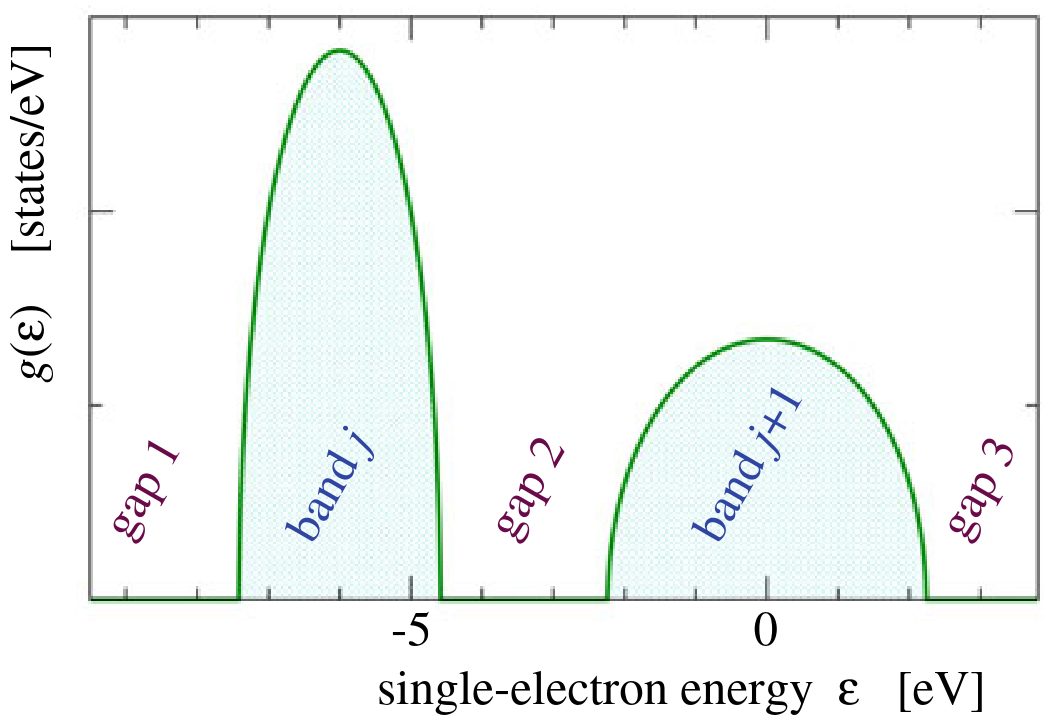
\includegraphics[width = 0.50 \textwidth]{band-dens.png}
	\caption{Sketch of the density of electronic states in a crystal.}
	\label{band-dens}
\end{figure}

Nei semiconduttori intrinseci, ovvero cristalli perfetti (a meno di impurità entropiche), la conducibillità elettrica è determinata dall'eccitazione termica di una parte di elettroni dalla banda di valenza a quella di conduzione. La densità numerica media di elettroni attivi è quindi:
\begin{equation*}
	\frac{[n_c]}{V} = \frac{1}{V} \int_{E_c}^\infty \dd E\, g(E) [n_E]_\text{F} = \frac{1}{V} \int_{E_c}^\infty \dd E \frac{g(E)}{e^{\beta (E - \mu)} + 1}
\end{equation*}
Uno sketch della densità di stati $ g(E) $ è riportato in Fig. \ref{band-dens}. Inoltre, si può approssimare il potenziale chimico nei pressi del punto medio della gap tra banda di valenza e banda di conduzione: essendo $ \Delta \gg k_\text{B} T $ (si noti che $ 1\ev $ corrisponde a circa $ 12'000 \,\text{K} $), allora $ E_c - \mu \approx \frac{\Delta}{2} \gg k_\text{B} T $. Si può dunque approssimare:
\begin{equation*}
	[n_E]_\text{F} = \frac{1}{e^{\beta (E - \mu)} + 1} \simeq e^{- \beta (E - \mu)} = e^{- \beta (E_c - \mu)} e^{- \beta (E - E_c)}
\end{equation*}
Il prefattore è piccolo ed indipendente dall'energia, dunque è uguale per tutti gli elettroni nella banda: la distribuzione elettronica si riduce quindi ad una distribuzione di Boltzmann (limite a bassa densità, in quanto il gas elettronico è estremamente rarefatto in questo contesto). Espandendo attorno al minimo della banda di conduzione, inoltre, si trova:
\begin{equation*}
	E = E_c + \frac{1}{2} \sum_{\alpha,\beta = 1}^3 \frac{\pa^2 E_{c,\ve{k}}}{\pa k_\alpha \pa k_\beta}\bigg\vert_{\ve{k}_\text{min}} (\ve{k} - \ve{k}_\text{min})_\alpha (\ve{k} - \ve{k}_\text{min})_\beta + \dots \,= E_c + \frac{\hbar^2}{2m_\text{eff}} \abs{\ve{k} - \ve{k}_\text{min}}^2 + \dots
\end{equation*}
L'energia d'eccitazione $ \Delta E = E - E_c $ ha quindi la forma dell'energia cinetica di una particella libera di massa $ m_\text{eff} $ (massa effettiva valutata in $ \ve{k}_\text{min} $) e numero d'onda calcolato rispetto a $ \ve{k}_\text{min} $. Di conseguenza, la densità degli stati di conduzione (a meno dello spin) è data dall'Eq. \ref{eq:en-deg}:
\begin{equation*}
	g_\text{tr}(E) = \frac{V m_\text{eff}^{3/2}}{\sqrt{2} \pi^2 \hbar^3} \sqrt{E - E_c}
\end{equation*}
Si può così esplicitare la densità numerica degli elettroni attivi:
\begin{equation*}
	\begin{split}
		\frac{[n_c]}{V}
		& = \frac{1}{V} \int_{E_c}^\infty \dd E \frac{g(E)}{e^{\beta (E - \mu) + 1}} \simeq \frac{e^{-\beta (E_c - \mu)}}{V} \int_{E_c}^\infty \dd E\, g_s g_\text{tr}(E) e^{-\beta (E - E_c)} \\
		& = e^{\beta (E_c - \mu)} \frac{\sqrt{2} m_\text{eff}^{3/2}}{\pi^2 \hbar^3} \int_0^\infty \dd E\, \sqrt{E} e^{-\beta E} = e^{\beta (E_c - \mu)} \frac{\sqrt{2} m_\text{eff}^{3/2}}{\pi^2 \hbar^3} \frac{\sqrt{\pi}}{2 \beta^{3/2}} = e^{\beta (E_c - \mu)} \left[ \frac{m_\text{eff} k_\text{B} T}{\sqrt[3]{2} \pi \hbar^2} \right]^{3/2}
	\end{split}
\end{equation*}
Per il silicio a $ T = 300 \,\text{K} $ si trova una densità numerica di elettroni attivi $ \sim 10^{15} \,\text{m}^{-3} $, 14 ordini di grandezza più piccola della tipica densità per i metalli. Si noti, però, che questa densità dipende esponenzialmente da $ T^{-1} $, ed infatti già a $ T = 600\,\text{K} $ si ha densità $ \sim 10^{29} \,\text{m}^{-3} $: a temperatura ambiente, i semiconduttori hanno resistività di vari ordini di grandezza maggiori rispetto ai metalli, ma la forte sensibilità dalla temperatura li rende ottimi sensori termici.

\paragraph{Semiconduttori estrinseci}

Dato che a temperatura ambiente la resistività dei semiconduttori intrinseci è talmente alta che si comportano da isolanti, per aumentarne la conduttività si aggiungono elementi di altro tipo in un processo detto \textit{drogaggio} (inserzione di impurità nel cristallo).










